\documentclass[brazil,pagestart=firstchapter]{abnt}

% This does not accept all Unicode chars (for instance: I²C gives an error)
%\usepackage[utf8]{inputenc}

% This adds support for Unicode chars.
\usepackage{ucs}
\usepackage[utf8x]{inputenc}
% But should be avoided:
% http://tex.stackexchange.com/questions/13067/utf8x-vs-utf8-inputenc

\usepackage[brazil]{babel}

% http://tex.stackexchange.com/questions/664/why-should-i-use-usepackaget1fontenc
% http://texblog.net/latex-archive/fonts/symbols/
\usepackage[T1]{fontenc}

% Use another font:
% http://tex.stackexchange.com/questions/553/what-packages-do-people-load-by-default-in-latex/951#951
%\usepackage{lmodern}

% 'microtype' improves LaTeX line-breaking algorithm by using
% microtypographic features of the font
% http://tex.stackexchange.com/questions/349/what-is-the-practical-difference-between-latex-and-pdflatex/358#358
\usepackage{microtype}


%%%%%%%%%%%%%%%%%%%%%%%%%%%%%%%%%%%%%%%%%%%%%%%%%%%%%%%%%%%%
% Acronyms and abbreviations

% Simple and effective acronym package:
\usepackage[printonlyused,withpage]{acronym}

% This one from abntex does not work correctly:
% http://comments.gmane.org/gmane.comp.tex.brazilian/13365
%\usepackage{tabela-simbolos}

% "nomencl" is quite annoying to use, specially when compared to "acronym".
% "nomencl" requires an external file and some extra commands.
% "acronym", on the other hand, just works out of the box!
%\usepackage{nomencl}
%\makenomenclature
% http://en.wikibooks.org/wiki/LaTeX/Indexing#Abbreviation_list
% http://franz.kollmann.in/latex/latex.html#abbr
% latexmk needs a custom dependency for this package
% http://magic.aladdin.cs.cmu.edu/2007/11/06/continuous-latex-compilation-using-latexmk/


%%%%%%%%%%%%%%%%%%%%%%%%%%%%%%%%%%%%%%%%%%%%%%%%%%%%%%%%%%%%
% Other packages

% http://en.wikibooks.org/wiki/LaTeX/Advanced_Mathematics
\usepackage{amsmath}
\DeclareMathOperator{\angulo}{ang}

% Adding \textsubscript{}
% LaTeX already has \textsuperscript, but lacks \textsubscript.
% http://en.wikibooks.org/wiki/LaTeX/Formatting#Text_mode_superscript_and_subscript
\usepackage{fixltx2e}

% Better handling of space after a custom command.
% http://tex.stackexchange.com/questions/17730/newcommand-and-spacing
\usepackage{xspace}

% This package detects footnotes that are split over several pages, and
% writes a warning to the log file.
\usepackage{fnbreak}

% http://tex.stackexchange.com/questions/32208/footnote-runs-onto-second-page
% http://www.tex.ac.uk/cgi-bin/texfaq2html?label=splitfoot
%\interfootnotelinepenalty=10000

% Avoid floats and figures from crossing a section boundary
% http://en.wikibooks.org/wiki/LaTeX/Floats,_Figures_and_Captions#Keeping_floats_in_their_place
\usepackage[section]{placeins}

% Required for including graphics
\usepackage{graphicx}

% Inserting PDF pages from other documents
\usepackage{pdfpages}

% SI Units
% https://bitbucket.org/josephwright/siunitx/issue/100/undefined-control-sequence-bit-and-byte
\usepackage{siunitx}
\sisetup{
	load-configurations = binary,
	per-mode = symbol,
	list-final-separator = { e },
	range-phrase = { a },
	output-decimal-marker = {,}
}
\DeclareSIUnit\gauss{G}

% To find the total number of pages
%\usepackage{lastpage}

%%%%%%%%%%%%%%%%%%%%%%%%%%%%%%%%%%%%%%%%%%%%%%%%%%%%%%%%%%%%
% Embedding source-code

%\usepackage{color}
%\usepackage{xcolor}

% LaTeX, as delivered, offers no means of handling bold "teletype" fonts
% http://www.tex.ac.uk/cgi-bin/texfaq2html?label=bold-extras
% http://tex.stackexchange.com/questions/33039/using-ttfamily-with-bfseries-or-how-to-enable-bold-in-fixed-width-font
% And the solution is to load another fixed-width font:
%\usepackage{courier}
%\usepackage{couriers}
%\usepackage{beramono}
% Either load all fonts from this pack:
\usepackage{txfonts}
% Or load only the typewriter one.
%\renewcommand{\ttdefault}{txtt}

% For inserting source-code
\usepackage{listings}

% Translating "Listing"
\renewcommand{\lstlistingname}{Listagem}

% Setting the default options
\lstset{
	basicstyle=\ttfamily\footnotesize,
	numberstyle=\scriptsize,
	numbers=left,
	escapeinside={(*@}{@*)},
	tabsize=4,
	breaklines=true,
	breakatwhitespace=true,
	showspaces=false,
	showstringspaces=false,
	showlines=false,
	captionpos=b
}
%	extendedchars=true,
%	inputencoding=utf8x,
%	numbersep=5pt,
%	frame=shadowbox,
%	frameround=rrrt,
%	rulecolor=\color{black},
%	rulesepcolor=\color{black},
% These don't seem to work if the caption is at the bottom
%	abovecaptionskip=\parskip,
%	belowcaptionskip=\parskip


% AVISO!!!  (copiado de outro projeto, mas não se aplica aqui)
% Dentro dos exemplos de código-fonte abaixo, coloquei um "tab" de
% indentação por estar dentro de um "frame", e "espaços" para a
% indentação do código de exemplo. Isto foi necessário porque os tabs
% estavam sendo ignorados dentro do códigos de exemplo.

\lstnewenvironment{ccode}[1][]
{\lstset{language=C,
	#1}
}{}

\lstnewenvironment{pythoncode}[1][]
{\lstset{language=Python,
	#1}
}{}

\lstnewenvironment{shellcode}[1][]
{\lstset{language=bash,
	#1}
}{}

% \begin{lstlisting}[caption={Useless code},label=useless]
% \end{lstlisting}


%%%%%%%%%%%%%%%%%%%%%%%%%%%%%%%%%%%%%%%%%%%%%%%%%%%%%%%%%%%%
% Table-related packages:

% For multirow cells inside tabular environments
%\usepackage{multirow}

% Longtable allows you to write tables that continue to the next page
%\usepackage{longtable}

% 'tabularx' package - simple column stretching
% http://en.wikibooks.org/wiki/LaTeX/Tables#The_tabularx_package_-_simple_column_stretching
%\usepackage{tabularx}

% 'booktabs' - Publication quality tables in LaTeX
%\usepackage{booktabs}

% Alternating row colors in tables
%\usepackage[table]{xcolor}
%\definecolor{tabular-odd-color}{gray}{0.90}
%\definecolor{tabular-even-color}{gray}{0.97}


%%%%%%%%%%%%%%%%%%%%%%%%%%%%%%%%%%%%%%%%%%%%%%%%%%%%%%%%%%%%
% Fancy headers (and footers)
% http://en.wikibooks.org/wiki/LaTeX/Page_Layout#Page_Styles
%\usepackage{fancyhdr}
%\pagestyle{fancy}
%
%% Headers and footers definition:
%\lhead{\includegraphics[height=21mm]{shared/2aliancas_h.pdf}}
%\chead{}
%% This \parbox is a hack to keep text aligned at top, but it's not the
%% only available solution:
%% http://tex.stackexchange.com/questions/2440/how-to-vertically-align-headers-footers-in-fancyhdr-package
%\rhead{\parbox[b][21mm][t]{0.65\textwidth}{\raggedleft\large\titletext \\[1em] \subtitletext}}
%\lfoot{}
%\cfoot{}
%\rfoot{Page \thepage{} of \pageref{LastPage}}
%
%\renewcommand{\headrulewidth}{0pt}  % Default is 0.4pt
%\renewcommand{\footrulewidth}{0pt}  % Default is 0pt


%%%%%%%%%%%%%%%%%%%%%%%%%%%%%%%%%%%%%%%%%%%%%%%%%%%%%%%%%%%%
% 'hyperref' for including hyperlinks to the PDF.
% It should be loaded last.
% http://en.wikibooks.org/wiki/LaTeX/Formatting#Typesetting_URLs
\usepackage{hyperref}
\hypersetup{
	pdfborder={0 0 0},
	hyperindex=false
}
% hyperindex=false is required by "tabela-de-simbolos"

% http://en.wikibooks.org/wiki/LaTeX/Labels_and_Cross-referencing#Issues_with_links_to_tables_and_figures_handled_by_hyperref
%\usepackage[all]{hypcap}


%%%%%%%%%%%%%%%%%%%%%%%%%%%%%%%%%%%%%%%%%%%%%%%%%%%%%%%%%%%%
% Custom commands
% http://tex.stackexchange.com/questions/1050/whats-the-difference-between-newcommand-and-newcommand

% http://tex.stackexchange.com/questions/24132/overline-outside-of-math-mode
\makeatletter
\newcommand*{\textoverline}[1]{$\overline{\hbox{#1}}\m@th$}
\makeatother

% http://tex.stackexchange.com/questions/15009/macros-for-common-abbreviations
\newcommand*{\eg}{e.g.\@\xspace}
\newcommand*{\ie}{i.e.\@\xspace}

\newcommand*{\VBUS}{V\textsubscript{BUS}\xspace}
\newcommand*{\VCC}{V\textsubscript{CC}\xspace}
\newcommand*{\VDD}{V\textsubscript{DD}\xspace}
\newcommand*{\GND}{GND\xspace}
% http://tex.stackexchange.com/questions/9691/avoid-hyphenation-in-2-d
\newcommand*{\VUSB}{\mbox{V-USB}\xspace}

\newcommand*{\resultadoimagens}[1]{
	\includegraphics[width=0.19\textwidth]{resultados/P30T30p0t0_a#1.png}
	\includegraphics[width=0.19\textwidth]{resultados/P45T45p0t0_a#1.png}
	\includegraphics[width=0.19\textwidth]{resultados/P60T60p0t0_a#1.png}
	\includegraphics[width=0.19\textwidth]{resultados/P75T75p0t0_a#1.png}
	\includegraphics[width=0.19\textwidth]{resultados/P85T85p0t0_a#1.png}
}

%%%%%%%%%%%%%%%%%%%%%%%%%%%%%%%%%%%%%%%%%%%%%%%%%%%%%%%%%%%%
% Other notes

% \linewidth is either \columnwidth in two-column mode or \textwidth in one-column mode.
% http://tex.stackexchange.com/questions/275/how-to-find-the-textwidth-in-two-column-mode/3531#3531

% Search-and-replace to add \textit to "mouse"
% :.,$s/\(textit{\)\@<!\<\(mouses\?\|joysticks\?\)\>/\\textit{\2}/gc


%%%%%%%%%%%%%%%%%%%%%%%%%%%%%%%%%%%%%%%%%%%%%%%%%%%%%%%%%%%%
% Some metadata

% This is used only by latex-beamer package:
%\title{Dispositivo apontador com interface USB usando magnetômetro}
%\author{Denilson Figueiredo de Sá}
%\date{2011-11-16}
%\institute{DCC/UFRJ}
%\keywords{AVR, USB, mouse, magnetometer}

\autor{Denilson Figueiredo de Sá}
\titulo{Dispositivo apontador com interface USB usando magnetômetro}
\orientador{Nelson Quilula Vasconcelos}
%\comentario{}
\instituicao{Departamento de Ciência da Computação \par Instituto de Matemática \par Universidade Federal do Rio de Janeiro}
\local{Rio de Janeiro - RJ, Brasil}
\data{16 de novembro de 2011}

% latex-beamer sets the pdftitle and pdfauthor automatically, but here we
% must explicitly run it:
\hypersetup{
	pdftitle={\ABNTtitulodata},
	pdfauthor={\ABNTautordata}
}

%%%%%%%%%%%%%%%%%%%%%%%%%%%%%%%%%%%%%%%%%%%%%%%%%%%%%%%%%%%%
\begin{document}

% The "abnt" class issues a warning:
%   pdfTeX warning (ext4): destination with the same identifier
%   (name{page.i}) has been already used, duplicate ignored
% This page has a solution (or workaround):
% http://en.wikibooks.org/wiki/LaTeX/Hyperlinks#Problems_with_Links_and_Pages
%\pagenumbering{roman}
% But, anyway, it's better to ignore that warning (or even better would be
% to report it to abntex maintainers).
% Instead of messing with page numbering, I've added pagestart=firstchapter
% option.


\capa

\folhaderosto


\begin{folhadeaprovacao}

\setlength{\ABNTsignthickness}{0.4pt}
\setlength{\ABNTsignskip}{2cm}
\hspace*{1cm}

\centerline{\textbf{\large \ABNTtitulodata}}

\bigskip
\bigskip

\centerline{\textbf{\ABNTautordata}}

\bigskip
\bigskip

Projeto Final de Curso submetido ao Departamento de Ciência da Computação
do Instituto de Matemática da Universidade Federal do Rio de Janeiro como
parte dos requisitos necessários para obtenção do grau de Bacharel em
Ciência da Computação.

Apresentado por:

\assinatura{\ABNTautordata}

Aprovado por:

\assinatura{Prof. Nelson Quilula Vasconcelos \\ Orientador}
\assinatura{Prof. Adriano Joaquim de Oliveira Cruz}
\assinatura{Profª. Silvana Rossetto}

\bigskip
\bigskip
\bigskip

\begin{center}
\ABNTlocaldata

\ABNTdatadata
\end{center}

\end{folhadeaprovacao}


% Colocar o Sumário aqui é muito bom, mas não é de acordo com a norma ABNT
% NBR 14724: informação e documentação: trabalhos acadêmicos: apresentação.
%\tableofcontents{}


%\pretextualchapter{Dedicatória}
% TODO: escrever dedicatória (opcional)

\pretextualchapter{Agradecimentos}

Agradeço aos professores do DCC/UFRJ, em especial aos professores
\textsc{Nelson Quilula Vasconcelos},
\textsc{Adriano Joaquim de Oliveira Cruz}, e
\textsc{Silvana Rossetto} por participarem deste projeto,
e aos professores
\textsc{João Carlos Pereira da Silva},
\textsc{Márcia Rosana Cerioli} e
\textsc{Monique Moura Carmona} pelo apoio durante esses anos de faculdade.

Agradeço aos amigos de faculdade, em especial
\textsc{Alexandre Araújo Moreira},
\textsc{Luana Pinto Araújo} e
\textsc{Priscila Neves Bilangieri} por toda a paciência e apoio nos
momentos em que mais precisei de ajuda.

Agradeço também ao amigo de faculdade
\textsc{Bruno Bottino Ferreira} pela paciência durante as semanas finais
deste projeto.

Agradeço aos amigos de trabalho, em especial
\textsc{Claudio Sá de Abreu} e
\textsc{Marcelo Salhab Brogliato} pelo apoio e pelo crescimento pessoal e
profissional que me proporcionaram.


\begin{resumo}
Este projeto tem como objetivo implementar um dispositivo apontador
compatível com um \textit{mouse} USB utilizando um microcontrolador AVR
ATmega8 de 8 bits e um magnetômetro. O dispositivo fruto deste projeto
permite o usuário controlar o ponteiro do mouse movendo um sensor no ar,
simplesmente apontando-o para a posição desejada na tela. É uma forma
bastante intuitiva de controlar o ponteiro em situações onde um
\textit{mouse} não é adequado. Pode também ser usado para fins de
acessibilidade, controlando o ponteiro através de movimentos da cabeça ou de
qualquer outra parte do corpo.
\end{resumo}

\begin{abstract}
This project implements a USB HID absolute pointing device using an ATmega8
AVR 8-bit microcontroller and a magnetometer. This device allows the user to
control the mouse pointer by just moving a sensor in the air, pointing it to
the desired screen position. It is a very intuitive way to control the
pointer whenever it is not appropriate to use a mouse. It can also be used
for accessibility, controlling the pointer by head movements, or movements
of any other part of the body.
\end{abstract}


\listoffigures

%\listoftables


% The following command does not work:
% \listadesiglas
% Instead, I'm using "acronym" package.

\pretextualchapter{Lista de Siglas}

\begin{acronym}[EEPROM]

\acro{ADC}{Analog-to-Digital Converter}
\acro{API}{Application Programming Interface}
\acro{BIOS}{Basic Input/Output System}
\acro{DIP}{Dual In-line Package}
\acro{EEPROM}{Electrically Erasable Programmable Read-Only Memory}
\acro{HID}{Human Interface Device}
\acro{I2C}[I²C]{Inter-Integrated Circuit}
\acro{ICSP}{In-Circuit Serial Programmer}
\acro{ISP}{In-System Programmer}
\acro{LCC}{Leaded Chip Carrier}
\acro{LED}{Light-Emitting Diode}
\acro{LKML}{Linux Kernel Mailing List}
\acro{NRZI}{Non-Return-to-Zero Inverted}
\acro{PCB}{Printed Circuit Board}
\acro{PDIP}{Plastic Dual In-line Package}
\acro{QFN}{Quad-Flat No-leads Package}
\acro{QFP}{Quad Flat Package}
\acro{ROM}{Read-Only Memory}
\acro{SCL}{Serial Clock}
\acro{SDA}{Serial Data}
\acro{SE0}{Single-Ended 0}
\acro{SE1}{Single-Ended 1}
\acro{SRAM}{Static Random-Access Memory}
\acro{TWI}{Two-Wire Interface}
\acro{USB-IF}{USB Implementers' Forum}
\acro{USB}{Universal Serial Bus}

\end{acronym}


\tableofcontents


\chapter{Introdução}
\label{cap:introducao}


\vfill{}
\begin{flushright}{}
``\emph{The world is moving so fast these days that the man who says it
can't be done is generally interrupted by someone doing it.}''\\
{\small Elbert Green Hubbard}
\end{flushright}{\small \par}
\vfill{}

Neste capítulo são apresentados a motivação e os objetivos deste projeto, uma
lista de trabalhos relacionados e a estrutura da monografia.
\newpage


\section{Motivação e objetivos}
\label{sec:motivacao}

Este projeto apresenta uma implementação de um dispositivo \acs{USB} do tipo
\textit{absolute pointing device} que pode ser utilizado para controlar o
ponteiro do \textit{mouse} na tela do computador seguindo os movimentos de
um sensor. Dentre outras aplicações, este dispositivo pode ser muito
conveniente em apresentações que usem um computador ligado a um projetor.

O sensor empregado neste projeto é um magnetômetro, também conhecido como
bússola digital, o qual permite medir a direção e a intensidade do campo
magnético. Desta forma, é possível saber a direção (em relação à Terra) para
onde o sensor está sendo apontado. A partir dessa informação é calculada
a posição desejada para o ponteiro do \textit{mouse}.

Todos os cálculos são realizados por um microcontrolador ATmega8, no qual
também foi implementado o protocolo \acs{USB} \acs{HID}. Assim, o
dispositivo fruto deste projeto pode ser usado em qualquer computador sem a
necessidade da instalação de \textit{drivers} específicos no sistema
operacional.

A ideia para este projeto surgiu da apresentação ``Google I/O 2011: The
Secrets of Google Pac-Man: A Game Show'', na qual o palestrante Marcin
Wichary utiliza um \textit{iPod touch}\footnote{
	\textit{iPod touch} é um reprodutor multimídia portátil bastante similar
	ao telefone celular \textit{iPhone}, porém sem todos os recursos deste.
	O \textit{iPod touch} possui um acelerômetro e um giroscópio embutidos,
	mas não possui um magnetômetro.
} preso ao seu pulso para controlar um objeto no telão através dos
movimentos de seu braço \cite{GoogleIO2011}. O software
que rodava no \textit{iPod touch} durante a palestra era uma página escrita
em HTML5 e JavaScript, a qual se comunicava com um servidor NodeJS através
de uma conexão Wi-Fi. Conforme ele movia seu braço, os dados do acelerômetro
eram enviados para o servidor, que por sua vez os repassava para o
computador que estava ligado ao projetor.

Um \textit{iPod touch} é um equipamento bastante poderoso, mas também é
relativamente grande e caro\footnote{
	R\$~729,00 no site do fabricante \cite{AppleStoreiPodTouch}.
}. Não é muito prático deixar um dispositivo desse tamanho preso ao braço ou
a qualquer outra parte do corpo. Além disso, não é possível controlar um
computador diretamente através dele, é necessário instalar tanto no
\textit{iPod} como no computador algum \textit{software} específico para
essa funcionalidade.

Diante dessas observações este projeto foi iniciado, objetivando ser mais
barato, menor e mais simples de usar.

Uma vez concluído e posteriormente refinado, este projeto pode ser aplicado
para diversos fins. Estas são algumas das aplicações possíveis:

\begin{itemize}
\item Pode ser utilizado durante apresentações, permitindo ao palestrante
apontar regiões do telão através do gesto natural de se apontar com a mão.
\item Pode ser utilizado em situações onde um \textit{mouse} não é viável,
situações onde não há um apoio para um \textit{mouse} convencional.
\item Pode ser utilizado em exposições interativas, entretenimento e jogos.
\item Pode ser utilizado por pessoas que não podem ou não conseguem
movimentar um \textit{mouse}. O pequeno sensor pode ser preso à cabeça ou
qualquer outra parte do corpo.
\end{itemize}

Todo o material desenvolvido neste projeto está também disponível
\textit{online} em repositórios Mercurial e Git: \\
\url{https://bitbucket.org/denilsonsa/atmega8-magnetometer-usb-mouse} \\
\url{https://github.com/denilsonsa/atmega8-magnetometer-usb-mouse}


\section{Trabalhos relacionados}
\label{sec:trabalhos_relacionados}


\subsection{Wiimote}
\label{sub:wiimote}

Wiimote é o nome dado aos controles do vídeo-game Wii, fabricado pela
Nintendo. É um controle sem fio com acelerômetro embutido, capaz de detectar
movimentos, e também funciona como um apontador dentro da interface do
vídeo-game, bastando apontá-lo para a tela. Para isso, é necessário colocar
acima ou abaixo da tela uma \textit{sensor bar}, que nada mais é do que um
conjunto de \acsp{LED} infravermelhos \cite{WikipediaWiimote}.

Cada Wiimote possui uma câmera infravermelha na sua região frontal. A
posição do ponteiro é calculada através da posição dos \acsp{LED}, capturada
pela câmera do controle.

O funcionamento esperado do dispositivo implementado neste projeto --
controlar o ponteiro na tela simplesmente apontando um dispositivo de
\textit{hardware} para a posição desejada -- é muito similar ao Wiimote,
embora com tecnologias distintas.


\subsection{SmartNav, TrackIR, HeadMouse}
\label{sub:naturalpoint}

A empresa NaturalPoint criou um produto chamado SmartNav \cite{SmartNav}
para controlar o ponteiro do \textit{mouse} através de gestos. O produto é
composto de uma câmera colocada acima do monitor e um software proprietário
para Windows ou Mac OS X. A câmera possui \acsp{LED} infravermelhos
embutidos e consegue captar os pontos onde essa luz foi refletida. O usuário
deve colar um pequeno pedaço de papel reflexivo em sua cabeça, boné, ou
qualquer outra parte do corpo. O software no computador, então, processa a
imagem da câmera e a transforma em movimentos do ponteiro do \textit{mouse}.

A mesma empresa também lançou um produto chamado TrackIR \cite{TrackIR} que
funciona de maneira similar, porém é voltado para o mercado de jogos. Neste
caso, em vez de controlar o ponteiro do \textit{mouse}, os movimentos da
cabeça são enviados diretamente para o jogo, onde são traduzidos para
movimentos da câmera virtual dentro do ambiente simulado. Para obter seis
graus de liberdade nos movimentos, o usuário precisa colocar na cabeça uma
armação contendo três pontos reflexivos ou três \acsp{LED} infravermelhos.

Ambos os produtos exigem que o usuário fique na frente de uma câmera e
exigem um software proprietário instalado e configurado na máquina. O
produto TrackIR está à venda a partir de US\$~99,95, enquanto o SmartNav
está à venda a partir de US\$~399,00

A empresa Origin Instruments tem um produto chamado HeadMouse
\cite{HeadMouse} cujo funcionamento é muito similar ao SmartNav, mas
não requer nenhum software instalado. Esse produto se identifica como um
\textit{mouse} \acs{USB} e portanto funciona em qualquer sistema. Está à
venda por US\$~995,00.


\subsection{Projetos baseados em acelerômetro}
\label{sub:acelerometro}

WiSHABI \cite{WiSHABI} é um projeto de dispositivo sem fio \acs{USB} que
pode funcionar como teclado ou \textit{mouse} e faz leituras a partir de um
acelerômetro. Foi implementado usando dois microcontroladores ATmega8.

``USB Wireless Tilt Mouse + Minesweeper'' \cite{USBWirelessTiltMouse} é um
outro projeto de \textit{mouse} sem fio baseado num acelerômetro. Utiliza
microcontroladores ATmega32 ou ATmega644.

TiltStick \cite{TiltStick} é um projeto que implementa um \textit{joystick}
\acs{USB} baseado em leituras de um acelerômetro.

Em comum, todos esses projetos usam microcontroladores de 8 bits da família
AVR e implementam um dispositivo \acs{USB} \acs{HID} através do
\textit{driver} V-USB.


\section{Estrutura da monografia}
\label{sec:estrutura_da_monografia}

O capítulo \ref{cap:componentes_e_protocolos} descreve os componentes e
protocolos usados para a realização deste trabalho.

O capítulo \ref{cap:hardware} descreve o \textit{hardware} do dispositivo.

O capítulo \ref{cap:software} descreve o \textit{firmware}
(\textit{software}) do dispositivo.

O capítulo \ref{cap:coordenadas} descreve o problema de transformação de
coordenadas, apresentando as abordagens experimentadas e seus resultados.

O capítulo \ref{cap:conclusoes} apresenta as conclusões deste
trabalho, com os resultados alcançados e as limitações encontradas, assim
como sugestões para trabalhos futuros.


%\subsection{\textit{Eye-tracking}}
%\label{sub:eyetracking}

% LC Technologies, Inc.
% http://www.eyegaze.com/content/assistive-technology
%
% Tobii Technology
% http://www.tobii.com/
%
% EyeTech Digital Systems, Inc.
% http://www.eyetechds.com/

% http://www.technologyreview.com/Infotech/18254/
% http://hci.stanford.edu/research/GUIDe/applications.html
% http://www.bltt.org/pointer/index.htm#gen9
% http://www.inference.phy.cam.ac.uk/dasher/SpecialNeeds.html
% http://www.inference.phy.cam.ac.uk/dasher/Headmouse.html


\chapter{Componentes e protocolos}
\label{cap:componentes_e_protocolos}


\vfill{}
\begin{flushright}{}
``\emph{I loved music, and in my ninth year at MIT, I decided to buy a hi-fi
set. I figured that all I needed to do was look at the specifications. So I
bought what looked like the best one, turned it on, and turned it off in
five minutes, the sound was so poor.}''\\
{\small Amar Gopal Bose}
% http://www.brainyquote.com/quotes/quotes/a/amarbose355388.html
\end{flushright}{\small \par}
\vfill{}

Neste capítulo são apresentados o microcontrolador ATmega8 e o sensor
HMC5883L, assim como os protocolos \acs{USB} e \acs{USB} \acs{HID}, usados
na comunicação do microcontrolador com o computador, e o protocolo
\acs{I2C}, usado na comunicação do microcontrolador com o sensor.
\newpage


\section{Microcontrolador ATmega8}
\label{sec:atmega8}

ATmega8 é um microcontrolador de 8 bits da família AVR, fabricado pela
\textit{Atmel Corporation}. Suas características principais são
\cite{ATmega8}:

\begin{itemize}
\item Arquitetura Harvard, com espaços de endereçamento distintos para
instruções e para variáveis.
\item \num{8192} bytes de memória \textit{Flash} para guardar o programa.
\item \num{512} bytes de memória \ac{EEPROM} para guardar parâmetros de
configuração do programa.
\item \num{1024} bytes de memória \ac{SRAM} volátil para as variáveis.
\item Voltagem de operação de \SIrange{4.5}{5.5}{\volt}.
\item Clock máximo de \SI{16}{\mega\hertz} usando um cristal externo.
\item Interface de comunicação serial I²C/TWI.
\item Disponível no encapsulamento PDIP\footnote{
	O encapsulamento do tipo \ac{PDIP}, também chamado de \ac{DIP}, é o
	ideal para se trabalhar numa protoboard, pois o circuito integrado pode
	ser diretamente encaixado nela.}
de 28 pinos, assim como QFP e QFN\footnote{
	Para o produto final, em ambiente de produção industrial, o ideal é usar
	um encapsulamento mais compacto, como \ac{QFP} ou \ac{QFN}}
de 32 pinos.
\end{itemize}

A arquitetura dos processadores AVR foi projetada em conjunto com os
desenvolvedores do compilador de C da \textit{IAR Systems}. Como
consequência, o conjunto de instruções do AVR foi pensado de modo a
minimizar o \textit{overhead} durante a execução de programas que tenham
sido escritos em linguagens de alto nível \cite{avr_iar_design}.

Além disso, as instruções são executadas num pipeline de dois estágios,
permitindo um desempenho máximo de uma instrução por ciclo de
\textit{clock}. Nem sempre esse desempenho é
alcançado, pois algumas instruções (como as que acessam a memória \ac{SRAM}
e os desvios) demoram pelo menos dois ciclos \cite{ATmega8}.

Todas as instruções da arquitetura AVR ocupam 16 ou 32 bits (2 ou 4 bytes).
Por esse motivo, a memória \textit{Flash} é endereçada por \textit{words} de
16 bits. Podemos dizer que o ATmega8 possui \num{8192} bytes de memória
\textit{Flash}, ou de maneira equivalente, \num{4096} \textit{words}.
A memória \ac{SRAM} e a memória \ac{EEPROM} são
endereçadas por bytes \cite{ATmega8}.

O microcontrolador ATmega8 inclui um módulo de comunicação serial \ac{I2C},
porém, para evitar problemas de patentes e licenças, a \textit{Atmel
Corporation} usa o nome \ac{TWI} para sua implementação dessa interface
\cite{avrlibctwi}.

Embora existam alguns modelos de microcontrolador AVR com controlador
\acs{USB} embutido \cite{atmel_avr_product_list}, o microcontrolador ATmega8
usado neste projeto não possui nenhum tipo de \textit{hardware} dedicado
para essa função. Para tal, foi usado um \textit{driver} que implementa o
protocolo \acs{USB} via software, diretamente no \textit{firmware} do
microcontrolador. Essa solução será descrita em mais detalhes na seção
\ref{sec:vusb}.


\section{Sensor HMC5883L}
\label{sec:sensor}

HMC5883L é um magnetômetro fabricado pela \textit{Honeywell}. Um
magnetômetro é também conhecido como ``bússola digital'' ou ``bússola
eletrônica''.

Esse sensor trabalha de \SIrange{2.16}{3.6}{\volt} e é capaz de medir a
intensidade do campo magnético usando o efeito magnetorresistivo em três
eixos perpendiculares (X, Y, Z) e converte essas medidas para um formato
digital através de um \ac{ADC} de 12 bits, chegando a uma precisão de
\SIrange{1}{2}{\degree}. Sua interface de comunicação é \ac{I2C}
\cite{HMC5883L}.

\begin{figure}[h]
\centering
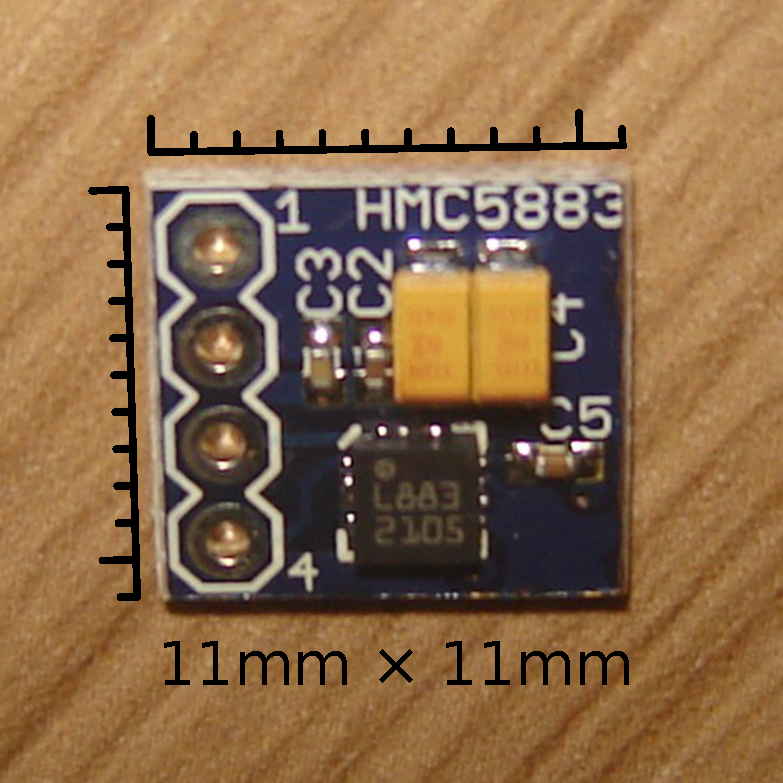
\includegraphics[width=0.45\textwidth]{img/sensor_front.pdf}
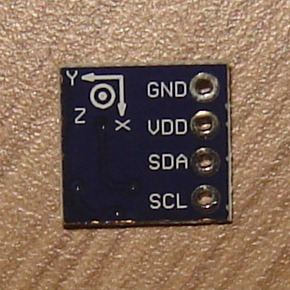
\includegraphics[width=0.45\textwidth]{img/sensor_back.jpg}
\caption{Fotos da PCB contendo o sensor}
\label{fig:sensor_photos}
\end{figure}

O circuito integrado possui encapsulamento \ac{LCC} e tem apenas
\SI[product-units=single]{3.0 x 3.0 x 0.9}{\milli\metre} de tamanho. É
impossível trabalhar manualmente com algo tão minúsculo, por isso foi
adquirida uma \ac{PCB} já contendo o sensor e alguns capacitores
\cite{ebay_HMC5883L}. Essa placa possui quatro contatos, sendo metade deles
para alimentação (\GND e \VDD) e a outra metade para comunicação \ac{I2C}
(SDA e SCL). Essa \ac{PCB} pode ser vista na figura \ref{fig:sensor_photos}.


\section{USB}
\label{sec:usb}

%\ac{USB} é um protocolo que foi desenvolvido a partir do ano de 1994 pelas
%empresas \textit{Compaq}, \textit{Hewlett-Packard}, \textit{Intel},
%\textit{Lucent}, \textit{Microsoft}, \textit{NEC} e \textit{Philips}. Foi
%motivado pela inexistência de um barramento bidirecional de baixo custo para
%periféricos de baixa e média velocidade, assim como a falta de flexibilidade
%dos barramentos até então existentes, os quais eram projetados para usos
%bastante específicos, sendo impossível reutilizá-los para outros
%periféricos \cite{usb20}.

A partir do ano de 1994, as empresas \textit{Compaq},
\textit{Hewlett-Packard}, \textit{Intel}, \textit{Lucent},
\textit{Microsoft}, \textit{NEC} e \textit{Philips} desenvolveram um
protocolo chamado \acf{USB}. Essa iniciativa foi motivada pela inexistência
de um barramento bidirecional de baixo custo para periféricos de baixa e
média velocidade. Além disso, a falta de flexibilidade dos barramentos até
então existentes não permitia reutilizá-los para outros periféricos, pois
eram projetados para usos bastante específicos \cite{usb20}.

A primeira versão do \ac{USB}, conhecida como ``USB 1.0'', foi oficialmente
lançada em janeiro de 1996 e definiu duas velocidades: \textit{low speed}
(\SI{1.5}{\mega\bit\per\second}) e \textit{full speed}
(\SI{12}{\mega\bit\per\second}). Alguns anos depois, em setembro de 1998, foi
lançada sua primeira revisão, ``USB 1.1'', que resolveu alguns problemas da
versão anterior mas não introduziu nenhuma mudança significativa.

A primeira grande revisão do protocolo foi lançada em abril de 2000, com o
nome de ``USB 2.0''. Esta versão introduziu uma terceira velocidade --
\textit{high speed} (\SI{480}{\mega\bit\per\second}) -- mas manteve total
compatibilidade com a revisão anterior do protocolo: dispositivos USB 1.x
funcionam em \textit{hosts} USB 2.0, e dispositivos USB 2.0 funcionam em
\textit{hosts} USB 1.x (porém limitados a \textit{full speed}).

\begin{figure}[h]
\centering
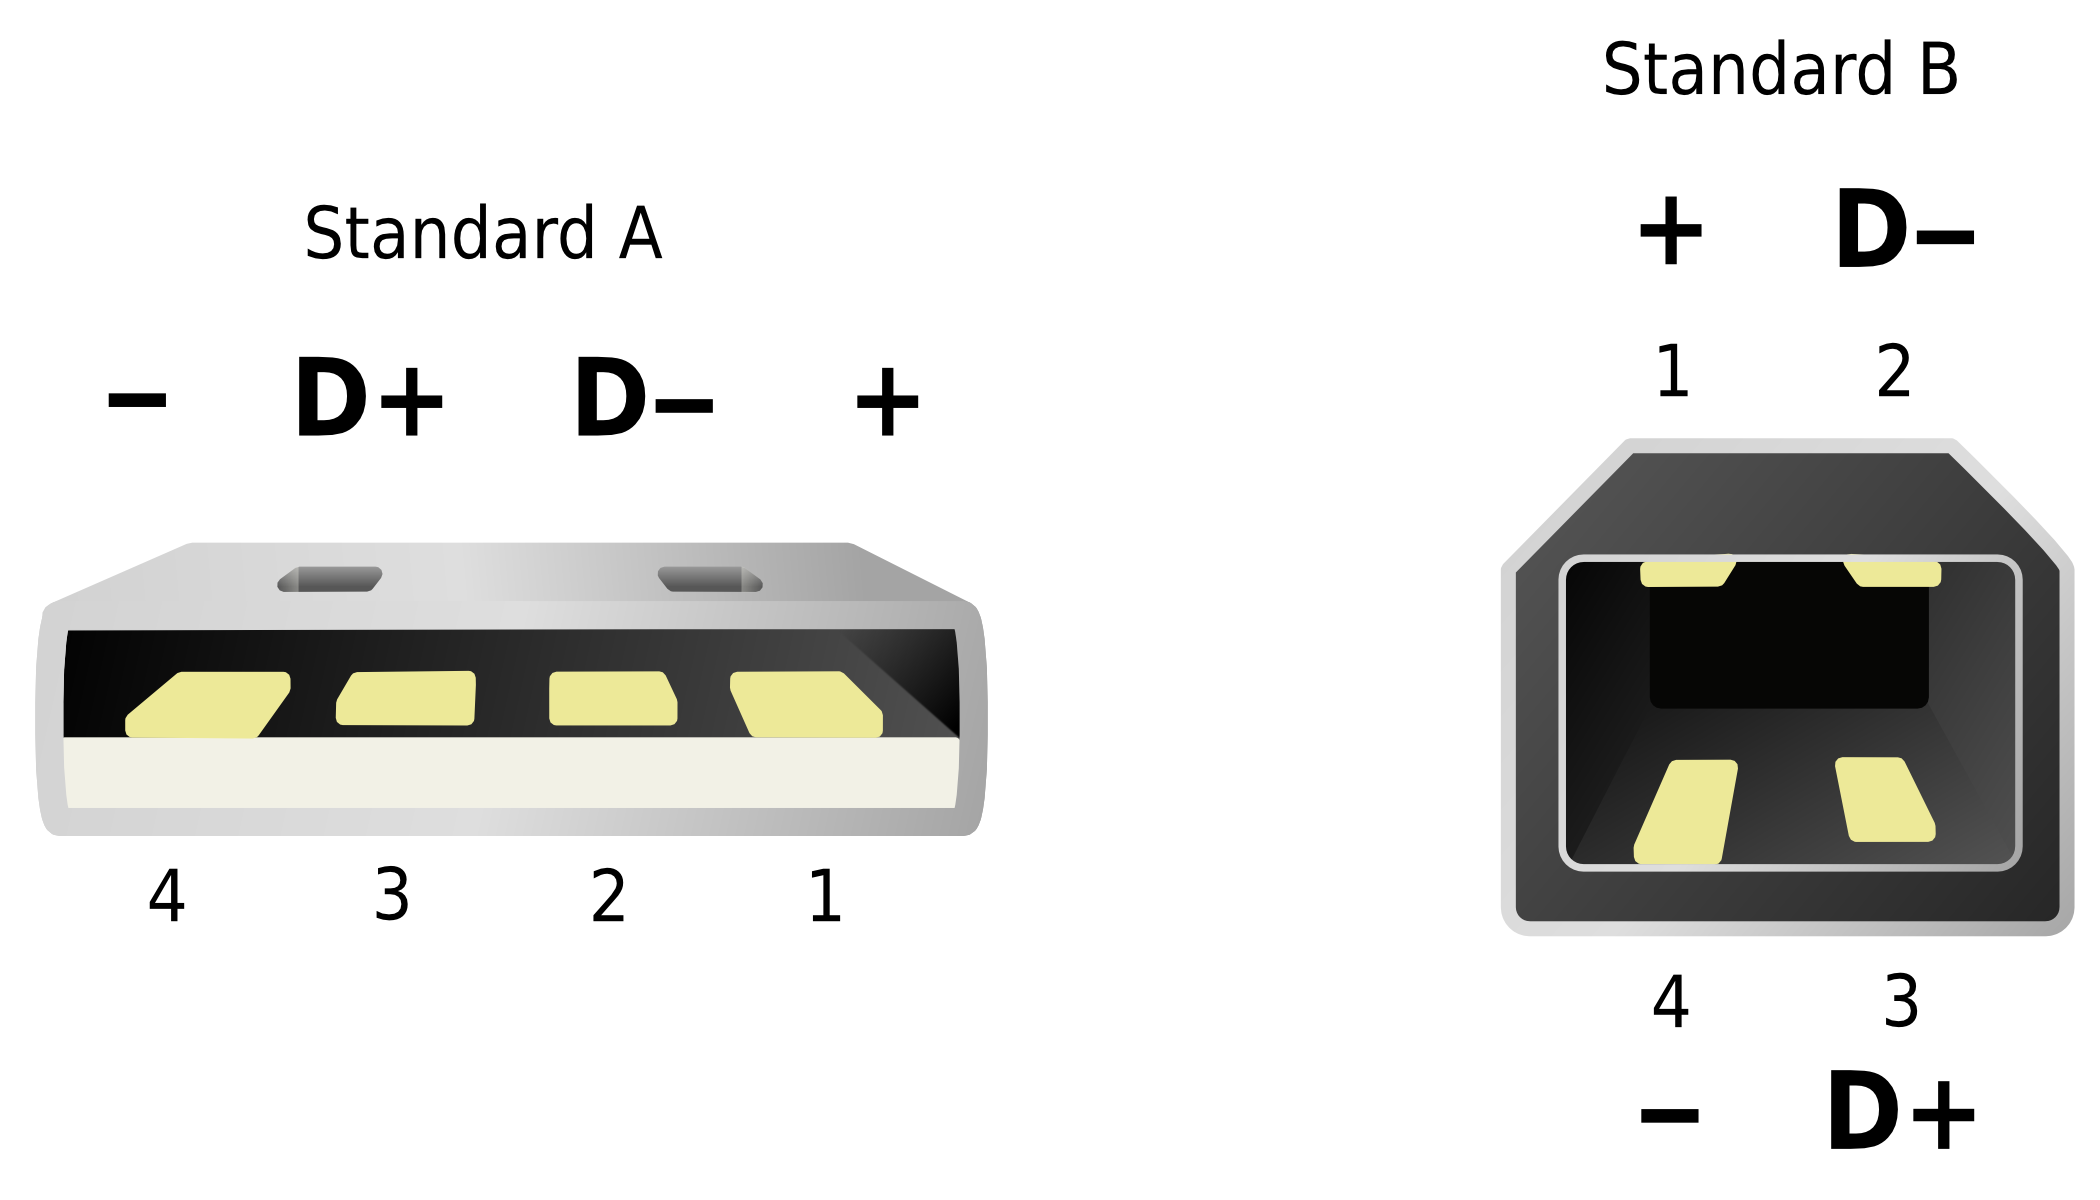
\includegraphics[width=0.5\textwidth]{img/USB.png}
\caption{Conectores do tipo A e do tipo B para USB 1.x/2.0}
\label{fig:usb_connectors}
\end{figure}

Uma conexão \ac{USB} é formada por quatro vias (conforme pode ser visto na
figura \ref{fig:usb_connectors}), sendo duas para alimentação (\VBUS =
\SI{+5}{\volt} e \GND) e duas para comunicação (D+ e D-). Os dados são
transmitidos usando a codificação \ac{NRZI} com \textit{bit stuffing} (um
``zero'' é inserido após seis bits ``um'' consecutivos)
\cite{usb20} \cite{usbinanutshell}.

A velocidade de um dispositivo é determinada por \textit{hardware}, de
acordo com a posição do resistor de \textit{pull-up}\footnote{
	Resistores de \textit{pull-up} ou de \textit{pull-down} servem para
	manter uma via de dados num nível lógico conhecido enquanto nenhuma
	transferência ocorre. Normalmente possuem um valor relativamente alto
	(de \SIrange{1.5}{10}{\kilo\ohm}) para drenar pouca corrente. Um
	resistor de \textit{pull-up} conecta a via ao \VDD e a mantém no nível
	lógico 1, enquanto um resistor de \textit{pull-down} conecta a via ao
	\GND e a mantém no nível lógico 0.}
nas vias de dados. Dispositivos
\textit{low speed} possuem um resistor de \textit{pull-up} ligado ao D-,
enquanto dispositivos \textit{full speed} possuem um resistor de
\textit{pull-up} ligado ao D+. Se não há nenhum resistor de
\textit{pull-up}, assume-se que não há nenhum dispositivo conectado
\cite{usb20} \cite{usbinanutshell}.

Dispositivos \textit{high speed}, introduzidos no \ac{USB} 2.0, inicialmente
se identificam como \textit{full speed} (com um resistor de \textit{pull-up}
ligado ao D+), mas removem o resistor após uma negociação realizada durante
o USB \textit{reset}, caso o \textit{host} também suporte \textit{high
speed}. Caso contrário, o resistor será mantido e o dispositivo funcionará
em \textit{full speed}. Essa negociação incial permite a compatibilidade
entre dispositivos USB 2.0 \textit{high speed} e \textit{hosts} USB 1.x
\cite{usb20} \cite{usbinanutshell}.

\begin{figure}[h]
\centering
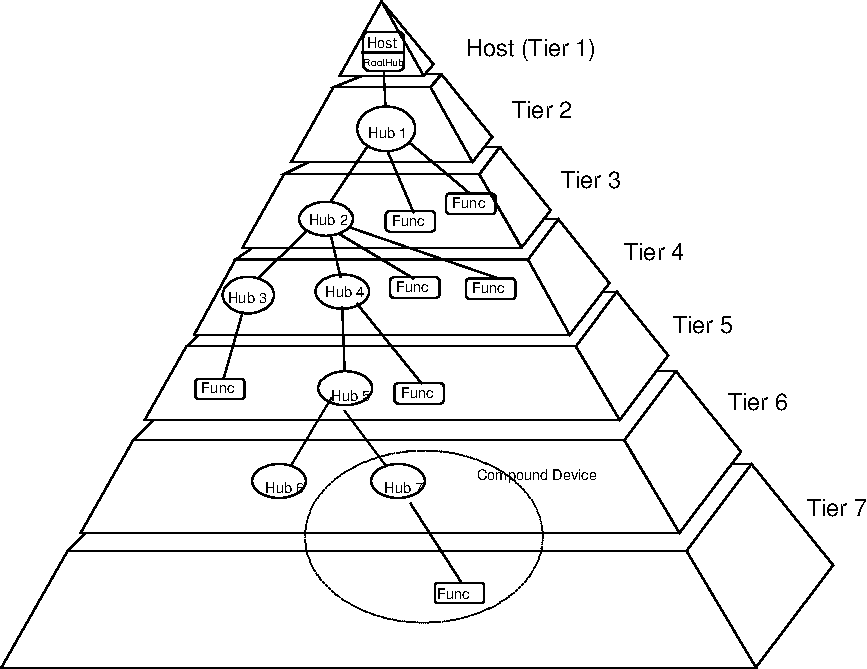
\includegraphics[width=0.75\textwidth]{img/usb_bus_topology.pdf}
\caption{Topologia do barramento USB}
\label{fig:usb_topology}
\end{figure}

A conexão de equipamentos \ac{USB} segue uma topologia de estrela em
camadas, que também pode ser entendida como uma árvore (conforme figura
\ref{fig:usb_topology}). No centro da estrela (ou na raiz da árvore) temos
obrigatoriamente o \textit{host}, que normalmente é um computador. Por
definição, o \textit{host} contém um \textit{root hub}. Cada cabo \ac{USB} é
uma conexão ponto-a-ponto que liga um \textit{hub} da camada imediatamente
acima a um dispositivo na camada imediatamente abaixo. Um dispositivo pode
ser um outro \textit{hub} ou então uma função. Por limitações de tempo de
propagação, o número máximo de camadas é sete, incluindo a camada que contém
o \textit{host} \cite{usb20}.

A especificação \ac{USB} define dois tipos de conectores (ilustrados na
figura \ref{fig:usb_connectors}). Um cabo \ac{USB} possui uma ponta de cada
tipo, sendo que o plugue do tipo A é conectado ao \textit{hub} da camada
acima, e o plugue do tipo B é conectado ao dispositivo da camada abaixo.
Posteriormente, foram também especificados conectores de tamanho mais
reduzido (Mini e Micro), mas os conceitos continuam os mesmos.

O protocolo de comunicação do \ac{USB} pode ser entendido como uma
arquitetura \textit{master/slave}, na qual o \textit{host} é o
\textit{master} e os dispositivos têm o papel de \textit{slave}. Só há um
\textit{host} por barramento \ac{USB} e ele é responsável por iniciar e
gerenciar cada transação. Como consequência, a maior parte da lógica está
centralizada no \textit{host}, simplificando bastante a implementação de
dispositivos que se conectam ao barramento \ac{USB} \cite{usbinanutshell}.

Em novembro de 2008, foi lançada a especificação do USB 3.0, que introduziu
uma quarta velocidade: \textit{super speed} (\SI{5}{\giga\bit\per\second}).
A quantidade de mudanças para suportar essa nova velocidade é grande e foge
do escopo deste trabalho.

% Não falei sobre:
% * Descriptors
% * * Device Descriptor
% * * Configuration Descriptor
% * * Interface Descriptor
% * * Endpoint Descriptor
% * * String Descriptor

\subsection{\textit{Endpoints}}
\label{sub:usb_endpoints}

Um \textit{endpoint} pode ser visto como um endereço lógico que pode receber
dados do \textit{host} ou enviar dados para ele. Todo dispositivo \ac{USB}
possui o \textit{endpoint~0}, usado pelo próprio protocolo para mensagens de
controle e de \textit{status} \cite{usbinanutshell}.

Além do \textit{endpoint~0}, um dispositivo \ac{USB} normalmente possui pelo
menos mais um \textit{endpoint}, usado para o objetivo fim do dispositivo.

Há quatro tipos de \textit{endpoints}: \cite{usbinanutshell}

\begin{description}
\item[Control] \hfill \\
	Bidirecional, usado durante a inicialização do dispositivo para comandos
	de controle do próprio protocolo \ac{USB}.
\item[Interrupt] \hfill \\
	Unidirecional, latência garantida.
\item[Isochronous] \hfill \\
	Unidirecional, latência e largura de banda garantidas, sem garantia de
	entrega, detecção de erros sem tentativa de reenvio. Apenas para
	dispositivos \textit{full speed} e \textit{high speed}.
\item[Bulk] \hfill \\
	Unidirecional, sem garantia de latência ou de banda, porém com entrega
	garantida e recuperação de erros. Apenas para dispositivos \textit{full
	speed} e \textit{high speed}.
\end{description}

\textit{Endpoints} do tipo \textit{bulk} são usados quando é importante
transmitir dados corretamente, sem preocupação com o tempo necessário para
concluir a transmissão. Dispositivos de armazenamento (como \textit{pen
drives}) e \textit{scanners} de fotos fazem uso deste tipo de
\textit{endpoint}.

\textit{Endpoints} do tipo \textit{isochronous} são usados principalmente
por dispositivos de \textit{streaming} multimídia (audio e vídeo), nos quais
há um fluxo constante de dados e o tempo de entrega é crítico.

\textit{Endpoints} do tipo \textit{interrupt} são usados para notificar o
\textit{host} de eventos do dispositivo, ou para notificar o dispositivo a
respeito de eventos do \textit{host}. Normalmente são mensagens curtas.
Dispositivos de interface com o usuário, descritos na seção
\ref{sec:usb_hid}, fazem uso deste tipo de \textit{endpoint}.

Quando as mensagens são enviadas do \textit{host} para o dispositivo, o
\textit{endpoint} é chamado de \textit{OUT}. Quando são do dispositivo para
o \textit{host}, o \textit{endpoint} é chamado de \textit{IN}.

É importante observar que um mesmo dispositivo pode ter múltiplos
\textit{endpoints} de tipos diferentes. Por exemplo, um \textit{scanner}
pode ter um \textit{endpoint} do tipo \textit{bulk-in} para transferir as
imagens e um \textit{endpoint} do tipo \textit{interrupt-in} para notificar
o \textit{host} quando o botão do dispositivo é apertado.


\section{USB HID}
\label{sec:usb_hid}

De modo a permitir a existência de dispositivos \textit{plug-and-play} --
que funcionam assim que são ligados ao \textit{host}, sem necessidade de
configurações feitas pelo usuário ou de instalação de drivers específicos --
foram definidas algumas classes de dispositivos. Por exemplo, os populares
\textit{pen drives}, que substituíram os disquetes e CDs regraváveis para
transferência de arquivos, pertencem à classe \textit{USB Mass Storage}, e
os sistemas operacionais modernos já incluem suporte nativo a dispositivos
dessa classe.

Dispositivos de interface com seres humanos fazem parte da classe
\textit{USB \acf{HID}} e abrangem principalmente teclados, \textit{mouses} e
\textit{joysticks}. No entanto, essa classe foi projetada de forma genérica
e inclui outros tipos de dispositivos com necessidades similares, tais como
medidores de temperatura, controles de um painel (botões, alavancas,
ajustes), volantes, pedais, leitores de códigos de barra, ou ainda novos
dispositivos que não foram previstos inicialmente na especificação
\cite{usbhid}.

A classe \ac{USB} \ac{HID} tem como objetivos ser compacta (para reduzir o
espaço necessário no \textit{firmware} do dispositivo), ser flexível e
extensível, ser genérica e auto-descritiva (de modo que cada dispositivo
descreva suas características de forma padronizada para o \textit{host}). O
driver da classe \ac{USB} \ac{HID}, presente no sistema operacional, é capaz
de se comunicar com qualquer dispositivo dessa classe \cite{usbhid}.

Eventos do dispositivo (\eg, um botão foi pressionado ou o \textit{mouse}
foi movimentado) são enviados ao \textit{host} através de um
\textit{interrupt-in endpoint}. Mensagens geradas pelo \textit{host} e que
devem ser enviadas para o dispositivo (\eg, acender ou apagar um dos
indicadores do teclado) podem utilizar um \textit{interrupt-out endpoint} ou
o \textit{control endpoint} \cite{usbhid}.

Essas mensagens enviadas ou recebidas pelo dispositivo são chamadas de
\textit{reports}. O formato delas é definido pelo próprio dispositivo,
através do \textit{report descriptor}, o qual é enviado ao \textit{host}
durante a negociação inicial do protocolo \ac{USB} \cite{usbhid}.

A primeira versão da especificação do \ac{USB} \ac{HID} foi lançada em
janeiro de 1996 (versão 1.0). Sua primeira revisão ficou disponível em abril
de 1999 (versão 1.1). Sua segunda revisão, que também é a mais recente, foi
lançada em junho de 2001 (versão 1.11). Apesar desta versão ter sido lançada
após o \ac{USB} 2.0, a especificação do \ac{USB} \ac{HID} menciona apenas as
duas velocidades de dispositivos presentes no \ac{USB} 1.x, e incorretamente
chama dispositivos \textit{full speed} de \textit{high-speed}
\cite{usbhid}.


\section{I²C}
\label{sec:i2c}

\acf{I2C} é um protocolo de comunicação serial bidirecional desenvolvido em
1982 pela \textit{Philips Semiconductors} (atual \textit{NXP
Semiconductors}). Foi projetado como um protocolo simples e eficiente para
comunicação entre circuitos integrados. Utiliza apenas duas vias: \ac{SCL} e
\ac{SDA} \cite{UM10204}.

A arquitetura do \ac{I2C} é baseada no modelo \textit{master/slave}, sendo
que qualquer um dos dispositivos do barramento pode assumir o papel de
\textit{master}, e inclusive o papel pode mudar ao longo do tempo. O
protocolo permite também múltiplos \textit{masters} no mesmo barramento
\cite{UM10204} \cite{ATmega8}. No entanto, para este trabalho
foi necessário apenas ligar dois dispositivos: o microcontrolador ATmega8
(funcionando sempre como \textit{master}) e o sensor HMC5883L (funcionando
sempre como \textit{slave}).

Tanto a via de dados \ac{SDA} como a via de \textit{clock} \ac{SCL} são
bidirecionais. O \textit{master} é responsável por gerar o sinal de
\textit{clock}, mas o dispositivo \textit{slave} pode esticar o período de
\textit{clock} em determinadas situações, indicando que ainda não está
pronto para responder \cite{UM10204}.

A comunicação no \ac{I2C} é baseada em bytes. O \textit{master} envia um
sinal de \textit{START}, seguido de um byte de endereço. Nesse byte, sete
bits, indicam o endereço do \textit{slave} e o oitavo bit indica o tipo de
comunicação (escrita ou leitura). Após a transmissão desse byte, o
\textit{master} libera a linha de dados e o \textit{slave} envia um bit zero
durante próximo pulso de \textit{clock}, sinalizando que recebeu o byte
(\textit{acknowledge}) \cite{AVR315}.

Logo após o byte de endereço, inicia-se a transmissão dos bytes de dados.
Caso seja uma escrita, o \textit{master} envia os bytes de dados exatamente
da mesma forma como enviou o byte de endereço, esperando pelo bit de
\textit{acknowledge} após cada byte enviado. Caso seja uma leitura, o
\textit{master} é responsável por gerar o \textit{clock} (conforme já
mencionado anteriormente), e o \textit{slave} envia um bit a cada pulso do
\textit{clock}. Após cada oito bits recebidos (ou seja, após cada byte), o
\textit{master} deve enviar um bit de \textit{acknowledge} para o
\textit{slave}. Em outras palavras, cada byte transmitido numa direção é
sempre seguido de um bit de \textit{acknowledge} transmitido na direção
contrária \cite{AVR315}.

O \textit{master} finaliza uma transmissão enviando um sinal \textit{STOP},
ou então enviando um novo sinal \textit{START} para iniciar uma nova
transmissão imediatamente (condição conhecida como \textit{REPEATED START})
\cite{ATmega8}.

Pode-se também observar que a quantidade total de bytes transferidos é uma
escolha do \textit{master}, e o \textit{slave} não tem como saber
inicialmente quantos bytes serão requisitados.


\chapter{Descrição do \textit{hardware}}
\label{cap:hardware}


\vfill{}
\begin{flushright}{}
``\emph{It's hardware that makes a machine fast. It's software that makes a
fast machine slow.}''\\
{\small Craig Bruce}
% http://www.brainyquote.com/quotes/quotes/c/craigbruce189163.html
\end{flushright}{\small \par}
\vfill{}

Neste capítulo são detalhados todos os componentes eletrônicos usados neste
projeto.
\newpage


\section{Visão geral do \textit{hardware}}
\label{sec:hardware_visao_geral}

O núcleo do circuito é o microcontrolador ATmega8, o qual é responsável por
ler os dados do sensor, fazer cálculos para converter os valores lidos, e
enviar as coordenadas via \ac{USB}.

A seção \ref{sec:hardware_microcontrolador} descreve como todos os
componentes são ligados ao microcontrolador.

A seção \ref{sec:hardware_usb} detalha a interface entre o microcontrolador
e a porta \ac{USB}.

A seção \ref{sec:hardware_sensor} detalha a interface entre o
microcontrolador e o sensor.

Um diagrama do circuito completo pode ser visto na figura
\ref{fig:circuito_completo}.


\section{Componentes ligados ao microcontrolador}
\label{sec:hardware_microcontrolador}

Um cristal de \SI{12}{\mega\hertz}, ligado aos pinos 9 e 10, define o
\textit{clock} do microcontrolador. O \textit{driver} usado para a
implementação do protocolo \ac{USB}, descrito na seção \ref{sec:vusb},
permite o uso de cristais de \SIlist[list-final-separator={ ou }]{12; 15;
16; 20}{\mega\hertz}. A escolha pelo cristal de \SI{12}{\mega\hertz} foi
arbitrária.

O pino 1 (\textoverline{RESET}) possui um resistor de \textit{pull-up}
(ligado ao \VCC) e um botão ligado ao \GND. Quando o botão é pressionado, o
nível lógico do pino cai para zero e o microcontrolador é reiniciado. Esse
botão de \textit{reset} se mostrou bastante útil durante o desenvolvimento,
mas não é necessário para o funcionamento deste projeto.

Há três \acp{LED} ligados aos pinos 11, 12 e 13 (PORTD5, PORTD6, PORTD7),
montados de modo a acender quando o valor lógico 1 é escrito. Foram usados
para fins de depuração, mas não são essenciais para o funcionamento deste
projeto.

Há três botões ligados aos pinos 23, 24 e 25 (PORTC0, PORTC1, PORTC2), e
ainda uma chave ligada ao pino 26 (PORTC3). Quando pressionados, o nível
lógico de cada pino cai para zero. Cada pino possui internamente um resistor
de \textit{pull-up}, o qual foi habilitado pelo \textit{firmware},
dispensando o uso de resistores externos.

Os pinos 17, 18 e 19 (MOSI, MISO, SCK), juntamente com o pino 1
(\textoverline{RESET}) são usados para \ac{ISP}. Por simplicidade e por
falta de necessidade, decidiu-se não usá-los para nenhuma outra função.

Por fim, os pinos 2 e 4 (PD0 e PD2) estão ligados às vias USB~D- e USB~D+, e
serão detalhados na seção \ref{sec:hardware_usb}; e os pinos 27 e 28 (SDA e
SCL) estão ligados ao sensor através de um barramento \ac{I2C}, e serão
detalhados na seção \ref{sub:hardware_sensor_i2c}.

\begin{figure}[h]
\centering
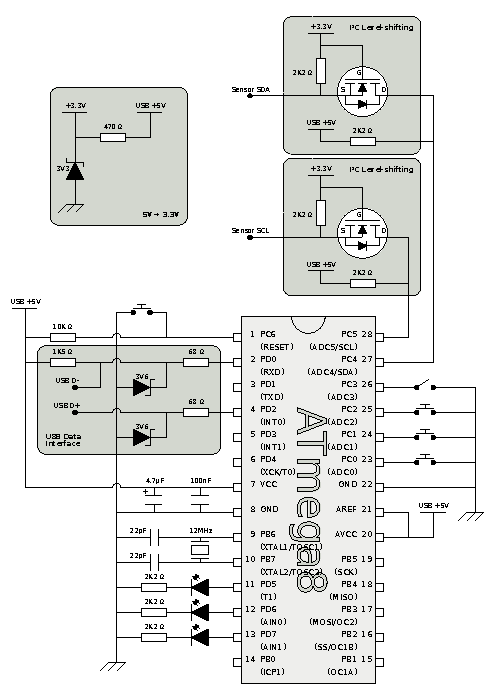
\includegraphics[width=1.0\textwidth]{img/AVR-magnetometer-usb-mouse.pdf}
\caption{Diagrama completo do circuito}
\label{fig:circuito_completo}
\end{figure}


\section{Interface USB}
\label{sec:hardware_usb}

Uma porta \ac{USB} fornece \SI{5}{\volt} na via \VBUS, porém a especificação
limita as vias de dados D+ e D- ao intervalo de \SIrange{2.8}{3.6}{\volt}
\cite{usb20}.

Uma solução seria usar um microcontrolador que possa funcionar a tensões
mais baixas e colocar um circuito para reduzir a alimentação para dentro do
intervalo desejado. Modelos mais recentes da linha AVR permitem o uso dessa
solução \cite{ATmega_newer_datasheets}. No entanto, o
microcontrolador ATmega8 usado neste projeto não trabalha com tensões
inferiores a \SI{4.5}{\volt} \cite{ATmega8}.

Uma outra solução é manter o microcontrolador alimentado com \SI{5}{\volt} e
adicionar um circuito para reduzir a saída dos pinos do AVR para a tensão
desejada. Esta foi a solução empregada neste projeto.

O circuito usado para reduzir a tensão nas linhas de dados segue o mesmo
esquema usado no projeto USBasp \cite{USBasp}, também disponível no arquivo
\texttt{circuits/with-zener.png} do \textit{driver} \VUSB \cite{VUSBdriver}.
É composto de um diodo Zener de \SI{3.6}{\volt} ligando a linha de dados ao
\GND e um resistor de \SI{68}{\ohm} entre o microcontrolador e o diodo
Zener.

Quando o microcontrolador escreve o nível lógico 1, seu pino sobe para
\SI{5}{\volt}. Como essa tensão é maior que a tensão de ruptura do Zener,
este começa a conduzir, limitando a tensão da linha de dados. A diferença de
$\num{5} - \num{3.6} = \SI{1.4}{\volt}$ fica no resistor, resultando numa
corrente de $\SI{1.4}{\volt} / \SI{68}{\ohm} = \SI{20.6}{\milli\ampere}$,
que é abaixo do limite de \SI{40}{\milli\ampere} para cada pino do
microcontrolador \cite{ATmega8}.

Além disso, conforme mencionado na seção \ref{sec:usb}, é preciso adicionar
um resistor de \textit{pull-up} à linha D-, indicando que este dispositivo
é \textit{low speed}. A especificação do USB 2.0 define que esse resistor
deve ter \SI{1.5}{\kilo\ohm} \cite{usb20}. O projeto USBasp, no
entanto, usa um resistor de \SI{2.2}{\kilo\ohm} \cite{USBasp}, que, mesmo
fora da especificação, também funcionou.

Por fim, para o funcionamento correto do \textit{driver} \VUSB, é necessário
que a linha USB~D+ esteja ligada ao pino INT0 do microcontrolador. Além
disso, é preciso que as duas vias de dados estejam ligadas a pinos que
pertençam à mesma porta do microcontrolador
\cite{VUSBdriver}. Portanto, a linha D+ foi ligada ao
pino 4 (PD2/INT0), e a linha D- foi ligada ao pino 2 (PD0).


\section{Interface com o sensor}
\label{sec:hardware_sensor}

\subsection{Alimentação}
\label{sub:hardware_sensor_alimentacao}

O sensor HMC5883L trabalha com alimentação de \SIrange{2.16}{3.6}{\volt}
\cite{HMC5883L}. Como a \ac{USB} fornece \SI{5}{\volt}, é necessário
adicionar um circuito para reduzir a tensão até um nível adequado.

A solução aqui empregada utiliza um diodo Zener de \SI{3.3}{\volt} e um
resistor de \SI{470}{\ohm} \cite{3vtipsandtricks}. É bastante similar àquela
descrita na seção \ref{sec:hardware_usb}, mudando apenas os valores dos
componentes.

O diodo Zener e o resistor estão ligados em série entre \VCC e \GND,
drenando constantemente uma corrente de $ (\SI{5}{\volt} - \SI{3.3}{\volt})
/ \SI{470}{\ohm} = \SI{3.6}{\milli\ampere} $ e mantendo a tensão de
\SI{3.3}{\volt} em relação ao \GND entre esses dois componentes.

Considerando que o sensor drena apenas \SI{0.1}{\milli\ampere} quando em
uso \cite{HMC5883L}, a queda de tensão na alimentação quando em carga
é desprezível, e portanto essa solução é bastante adequada para este
propósito.

\subsection{Barramento I²C}
\label{sub:hardware_sensor_i2c}

Se o microcontrolador e o sensor trabalhassem na mesma tensão, o barramento
\ac{I2C} seria apenas um par de fios ligando os pinos correspondentes dos
dois componentes, e dois resistores de \textit{pull-up}, um em cada fio.

Todavia, os dois componentes não trabalham na mesma tensão. A primeira
abordagem para este problema é verificar em suas especificações elétricas se
as tensões de cada um estão dentro da faixa aceitável para o outro
\cite{AN97055}. A tensão máxima de alimentação para o sensor é de
\SI{3.6}{\volt} \cite{HMC5883L}, e tensão máxima tolerada no pino de
alimentação é de \SI{4.8}{\volt} \cite{HMC5883L}, que é abaixo da
tensão de \SI{5}{\volt} do microcontrolador. Isso significa que não é
prudente ligar os dois componentes diretamente.

Neste caso, faz-se necessário adicionar um circuito para converter o nível
lógico 1 entre \SI{5}{\volt} e \SI{3.3}{\volt}. Essa conversão precisa
funcionar nas duas direções, pois o barramento é bidirecional.

A solução adotada utiliza dois resistores de \textit{pull-up} e um
transistor MOSFET de canal N para cada uma das vias do barramento. É uma
solução proposta pela própria \textit{Philips/NXP}, desenvolvedora do padrão
\ac{I2C} \cite{AN97055} \cite{AN10441}. Vários modelos diferentes de
transistor MOSFET podem ser usados para este fim. Neste projeto, foi usado o
modelo 2N7000. Os resistores de \textit{pull-up} usados foram de
\SI{2.2}{\kilo\ohm}.

Para entender como essa solução funciona, é preciso analisá-la em três
estados: \cite{AN97055} \cite{AN10441}

\begin{description}
\item[Nenhum dos dois dispositivos está puxando o barramento para zero] \hfill \\
	O lado de baixa tensão está em \SI{3.3}{\volt} devido ao resistor de
	\textit{pull-up}. A diferença de potencial entre os terminais
	\textit{gate} e \textit{source} do transistor é zero, e portanto ele não
	está conduzindo. Desta forma, o lado de tensão mais alta está em
	\SI{5}{\volt} devido ao resistor de \textit{pull-up}. Neste estado, os
	dois lados do barramento estão no nível lógico 1, apesar das tensões
	diferentes.

\item[O dispositivo de menor tensão está puxando o barramento para zero] \hfill \\
	A diferença de potencial entre os terminais \textit{gate} e
	\textit{source} é \SI{3.3}{\volt}, e o transistor entra em condução. O
	lado de tensão mais alta é também puxado para zero, através do
	transistor em condução.

\item[O dispositivo de maior tensão está puxando o barramento para zero] \hfill \\
	O lado de menor tensão é também puxado para baixo através do diodo
	interno do transistor MOSFET. Isso ocorre até que a diferença de potencial
	entre \textit{gate} e \textit{source} fique grande o suficiente, quando
	então o transistor entra em condução e o lado de menor tensão é puxado
	para zero através do transistor.

\end{description}


\chapter{Descrição do \textit{software}}
\label{cap:software}


\vfill{}
\begin{flushright}{}
``\emph{Premature optimization is the root of all evil.}''\\
{\small Donald Ervin Knuth}
% http://en.wikiquote.org/wiki/Donald_Knuth
\end{flushright}{\small \par}
\vfill{}

Neste capítulo é detalhado o \textit{firmware} deste projeto, assim como o
ambiente de desenvolvimento e algumas das dificuldades encontradas.
\newpage


\section{Visão geral do \textit{software}}
\label{sec:software_visao_geral}

Essencialmente, o trabalho do microcontrolador deste projeto é receber
medições do sensor, aplicar um algoritmo de transformação de coordenadas e
enviar para o computador as novas coordenadas do ponteiro. Para que isso
pudesse ser alcançado, o \textit{firmware} foi dividido em três grandes
partes.

A primeira parte é a comunicação com o sensor, descrita nas seções
\ref{sec:twi} e \ref{sec:software_sensor}.

A segunda parte é transformar os medições do sensor em coordenadas na tela
do computador. Um estudo das diferentes abordagens para esse problema e seus
resultados é apresentado no capítulo \ref{cap:coordenadas}.

A terceira parte é a comunicação com o computador, alcançada através da
implementação de um \ac{USB} \ac{HID} e descrita nas seções de
\ref{sec:vusb} a \ref{sec:mouse}.


\section{Ambiente de desenvolvimento}
\label{sec:software_ambiente}

O \textit{firmware} deste projeto foi desenvolvido em ambiente Linux x86\_64,
utilizando o compilador AVR-GCC versão 4.5.3, a biblioteca AVR-Libc versão
1.7.0 e as ferramentas do projeto Binutils versão 2.21.1. O código-fonte foi
escrito na linguagem C e é facilmente portável para outros
microcontroladores da família AVR. Para gravação do \textit{firmware} no
microcontrolador, foi usado o programa AVRDUDE.

Todo o ambiente de desenvolvimento usado (AVR-GCC, Binutils, AVR-Libc,
AVRDUDE) é composto por \textit{software} livre e está disponível para os
principais sistemas operacionais (FreeBSD, Linux, Mac OS X e Windows)
\cite{avrlibcoverview}.

O \textit{firmware} deste projeto pode ser compilado em qualquer sistema
operacional que tenha as ferramentas citadas, mesmo em outras versões,
embora alguns ajustes no Makefile possam ser necessários.


\section{\textit{Boot loader}}
\label{sec:bootloader}

Durante o início do projeto, o ciclo de desenvolvimento podia ser resumido
nestas etapas:

\begin{enumerate}
\item Compilar o código-fonte.
\item Desconectar a \textit{protoboard} da \ac{USB}.
\item Conectar o gravador de AVR na \ac{USB}.
\item Gravar a nova versão do \textit{firmware}.
\item Desconectar o gravador de AVR.
\item Reconectar a \textit{protoboard} na \ac{USB}.
\end{enumerate}

Rapidamente esse processo se mostrou bastante demorado e ineficiente,
atrasando os testes e a depuração do código recém-escrito, e portanto
atrasando o desenvolvimento. Além disso, também causava um desgaste mecânico
desnecessário na porta \ac{USB}. Embora esse desgaste seja desprezível a
curto prazo, poderia se tornar um problema real para projetos de longo
prazo.

Visando agilizar e simplificar o ciclo de desenvolvimento, foi gravado um
\textit{boot loader} na região de \textit{boot} do microcontrolador.

Foi usado o USBaspLoader \cite{USBaspLoader} como \textit{boot loader}. Ele
foi escolhido por ser \textit{open source} e por também usar o
\textit{driver} \VUSB, o qual será descrito em mais detalhes na seção
\ref{sec:vusb}.

Um \textit{boot loader} é gravado nos endereços mais altos da memória
\textit{Flash}. O microcontrolador ATmega8 tem suporte a \textit{boot
loaders} de tamanhos \numlist{256;512;1024;2048} bytes
\cite{ATmega8}. Após compilado, o USBaspLoader possui \num{2028}
bytes, e portanto ocupa os \num{2048} bytes superiores da memória
\textit{Flash}.

Logo após um \textit{reset}, o ATmega8 normalmente começaria a execução do
programa a partir do endereço mais baixo da memória. No entanto, quando se
ativa o \textit{boot loader} (através dos \textit{fuse bits} do
microcontrolador \cite{ATmega8}), a execução começa no endereço da
região de \textit{boot}.

Portanto, ao iniciar o microcontrolador, o USBaspLoader é executado antes do
\textit{firmware} principal. Se uma determinada condição (configurável) for
verdadeira, então o USBaspLoader assume o controle e se identifica como um
gravador USBasp\footnote{
	USBasp é um gravador de AVR com conexão USB que é implementado usando um
	microcontrolador ATmega8 ou similar \cite{USBasp}.
}.
Caso essa condição seja falsa (antes ou durante a execução do USBaspLoader),
então o \textit{firmware} principal é executado.

Com o uso deste \textit{boot loader}, o ciclo de desenvolvimento foi
reduzido para:

\begin{enumerate}
\item Compilar o código-fonte.
\item Deixar ligada a chave conectada ao pino 26 (PORTC3) do
microcontrolador.
\item Apertar o botão de \textit{reset}.
\item Gravar a nova versão do \textit{firmware}.
\end{enumerate}

Após receber uma nova versão do \textit{firmware} principal, o USBaspLoader
automaticamente inicia a execução desse \textit{firmware} recém-gravado.

Com o uso de um \textit{boot loader}, o ciclo de desenvolvimento tornou-se
notavelmente mais rápido e dinâmico. Testar mudanças no \textit{firmware}
passou a ser fácil, e os testes se tornaram mais frequentes.

Como desvantagem, o espaço disponível na memória \textit{Flash} do
microcontrolador foi reduzido de \num{8192} para \num{6144} bytes.


\section{Comunicação I²C/TWI}
\label{sec:twi}

O microcontrolador ATmega8 possui um \textit{hardware} dedicado para
comunicação \ac{I2C} (chamada de \ac{TWI}, conforme citado na seção
\ref{sec:atmega8}). No entanto, seu uso é relativamente burocrático, tendo
que implementar uma máquina de estados para gerenciar os registradores do
módulo de \ac{TWI} e a transmissão de dados \cite{ATmega8}. O
exemplo de código disponível na página 170 do \textit{datasheet} do ATmega8
utiliza a técnica de \textit{busy-wait} e não é adequado para o firmware
deste projeto.

De maneira geral, a técnica de \textit{busy-wait} (espera ocupada) deve
ser evitada porque bloqueia a execução do restante do código por tempo
indeterminado, durante o qual nenhum tipo de trabalho útil pode ser
realizado. Uma das possíveis consequências é causar um \textit{watchdog
reset}, reiniciando a execução do código do \textit{firmware}. Além disso,
a espera ocupada não garantiria que a função \texttt{usbPoll()} fosse
chamada em intervalos menores que \SI{50}{\milli\second}, conforme descrito
na seção \ref{sub:vusb_config}.

Reconhecendo a dificuldade de usar esse módulo de maneira eficiente, a
própria \textit{Atmel} publicou um documento e o código-fonte de um
\textit{driver}\footnote{
	Neste contexto, ``\textit{driver}'' significa um pedaço de
	\textit{software} dentro do \textit{firmware} que controla um módulo de
	hardware do microcontrolador. Não confundir com \textit{drivers} do
	sistema operacional.}
que utiliza o módulo \ac{TWI} de maneira mais eficiente \cite{AVR315}.

Para este projeto, foi usado o \textit{driver} disponível na
\textit{application note} ``AVR315: Using the TWI module as I²C master''.
Seu funcionamento é baseado em interrupções, e portanto pode realizar a
transmissão de vários bytes de maneira assíncrona (não-bloqueante), uma
característica altamente desejável. A rotina de tratamento da interrupção
basicamente implementa uma máquina de estados \cite{AVR315}.

O \textit{driver} possui um \textit{buffer} interno para armazenar os dados
a serem enviados ou os dados sendo recebidos. O tamanho desse
\textit{buffer} é configurável em tempo de compilação, através da linha:

\begin{ccode}[numbers=none]
#define TWI_BUFFER_SIZE     7
\end{ccode}

O código-fonte estava originalmente escrito para o compilador IAR. Adaptá-lo
para o compilador GCC foi uma tarefa bastante simples, bastando apenas
trocar os cabeçalhos e trocar a sintaxe da declaração da rotina de
interrupção \cite{avrlibcporting}.

\begin{ccode}[numbers=none, multicols=2, float=h]
// IAR:
#include "ioavr.h"
#include "inavr.h"
// GCC:
#include <avr/io.h>
#include <avr/interrupt.h>
\end{ccode}

\begin{ccode}[numbers=none, multicols=2, float=h]
// IAR syntax:
#pragma vector=TWI_vect
__interrupt void TWI_ISR(void)
{
  ...
}
// GCC syntax:
ISR(TWI_vect)
{
  ...
}

\end{ccode}


\section{Comunicação com o sensor}
\label{sec:software_sensor}

O sensor HMC5883L possui treze registradores de 8 bits que podem ser
acessados pela comunicação serial, mais um registrador interno
chamado de \textit{address pointer}, o qual aponta para algum dos outros
registradores e cujo valor não pode ser lido \cite{HMC5883L}.

Quando o \textit{master} inicia uma escrita, o primeiro byte recebido pelo
sensor é considerado o endereço de um registrador, e esse endereço é salvo
no \textit{address pointer}. Caso um segundo byte seja recebido, esse valor
é salvo no registrador apontado pelo \textit{address pointer}.

Assim, para escrever num dos registradores de configuração do sensor, o
\textit{firmware} do microcontrolador prepara um vetor de três bytes: o
endereço do sensor (juntamente com o bit que define uma operação de
escrita), o número do registrador de configuração que será modificado, e o
valor a ser escrito no registrador. Esse vetor é repassado ao
\textit{driver} de \ac{TWI} (descrito na seção \ref{sec:twi}), o qual copia
esses bytes para um \textit{buffer} interno e inicia a comunicação
assincronamente.

Quando o \textit{master} inicia uma leitura, o sensor envia um byte com o
valor contido no registrador apontado pelo \textit{address pointer} e
incrementa o \textit{address pointer} para apontar para o próximo
registrador. Caso outro byte seja requisitado (ainda na mesma transmissão,
ou em outra transmissão), o processo se repete, enviado o valor contido no
registrador apontado pelo \textit{address pointer} e incrementando-o. Desta
forma, é possível ler o conteúdo de vários registradores adjacentes de
maneira bem eficiente, com \textit{overhead} de comunicação mínimo.

No entanto, a implementação do sensor não é perfeita, e em certos casos o
auto-incremento do \textit{address pointer} não funciona como esperado. Por
exemplo, uma tentativa de ler todos os registradores (usando o
auto-incremento para iterar automaticamente por todos eles) retorna valores
diferentes (e inválidos) daqueles retornados por leituras individuais. De
maneira geral, o auto-incremento funciona corretamente apenas para a leitura
dos três registradores de identificação do sensor e para a leitura dos seis
registradores de dados, não atrapalhando o uso normal do sensor.

Para ler os valores X, Y, Z do sensor, o microcontrolador começa realizando
uma escrita no sensor, enviando o valor \texttt{0x03} como endereço do
registrador. A seguir, realiza uma leitura de seis bytes consecutivos. Por
fim, esses seis bytes lidos são convertidos numa \texttt{struct} de três
variáveis inteiras de 16 bits.

\subsection{Configuração do sensor}
\label{sub:software_sensor_config}

Durante a inicialização do \textit{firmware} do microcontrolador, os
registradores de configuração do sensor são escritos.

O sensor foi configurado para atualizar os registradores de dados 75 vezes
por segundo, sendo que cada valor é a média de oito amostras. O ganho do
sensor foi configurado para ±\SI{1.3}{\gauss}, o que corresponde a
\num{1090} bits por gauss\footnote{
	O símbolo \si{\gauss} corresponde à unidade de densidade de fluxo
	magnético ``gauss'' \cite{SI}. O \textit{datasheet} do sensor,
	no entanto, utiliza Ga como símbolo para essa unidade.
}, ou \SI{0.92}{\milli\gauss} por bit. Este ganho foi escolhido por permitir
a maior precisão possível das medidas sem causar \textit{overflow} no
sensor.

O sensor foi configurado para o modo de medição contínua, \ie, está
continuamente medindo o campo magnético e atualizando os registradores de
dados (75 vezes por segundo), mesmo que o microcontrolador não faça a
leitura dessas medidas.

Por limitação do sensor, o modo de medição contínua permite obter medições a
uma taxa máxima de \SI{75}{\hertz}. Apesar disso, é possível obter medições
a até \SI{160}{\hertz} se for configurado para o modo de medições
individuais e o pino DRDY for monitorado \cite{HMC5883L}. Este pino
normalmente fica no nível lógico 1, porém cai para 0 por
\SI{250}{\micro\second} assim que uma nova medida é colocada nos
registradores de dados \cite{HMC5883L}.  Portanto, seria possível ligar esse
pino DRDY a algum dos pinos de interrupção do microcontrolador e escrever
uma rotina que leia os dados e inicie a próxima medição.

Todavia, a \ac{PCB} usada neste projeto (figura \ref{fig:sensor_photos}) não
possui um contato para o pino DRDY, e portanto não foi possível se
aproveitar dessa técnica.


\section{\textit{Driver} \VUSB}
\label{sec:vusb}

O \textit{driver} \VUSB foi desenvolvido pela \textit{Objective Development
Software GmbH.} e é uma implementação em \textit{software} do protocolo
\ac{USB}, funcionando em diversos microcontroladores da família AVR que não
possuem um controlador \ac{USB} embutido \cite{VUSBdriver}.

Por ser implementado em \textit{software}, o tempo de execução das rotinas
do \textit{driver} é crucial, e essas rotinas foram implementadas (pelos
autores do \textit{driver}) em \textit{assembly} para \textit{clocks} de
\SIlist[list-final-separator={ ou }]{12; 15; 16; 20}{\mega\hertz} usando
cristal, ou \SIlist[list-final-separator={ ou }]{12.8; 16.5}{\mega\hertz}
usando o oscilador interno do microcontrolador. Não é possível usar o
\textit{driver} com frequências diferentes destas \cite{VUSBdriver}.

Apesar das rotinas internas estarem escritas em \textit{assembly}, o
\textit{driver} disponibiliza uma \ac{API} bastante simples em linguagem C.

O \textit{driver} implementa um dispositivo \ac{USB} 1.1 \textit{low speed},
mas possui algumas limitações. Uma delas é assumir que não há erros durante
a comunicação, pois não há tempo de CPU suficiente para implementar checagem
de erros via \textit{software}. Além disso, as características elétricas dos
pinos do microcontrolador não atendem estritamente a especificação \ac{USB}
\cite{VUSBdriver}.

A especificação \ac{USB} também define que os dispositivos devem implementar
um modo \textit{suspend}, no qual não devem consumir mais que
\SI{500}{\micro\ampere} \cite{usbinanutshell}. O \textit{driver} não
implementa esse modo, mas explica em linhas gerais como seria possível
implementá-lo \cite{VUSBdriver}. Para este projeto, não foi
implementado o suporte ao modo \textit{suspend}, pois não é uma tarefa
trivial e está fora do escopo deste trabalho.

Considerando as limitações citadas nos parágrafos anteriores, o dispositivo
fruto deste projeto não é totalmente conformante com a especificação
\ac{USB}, mas isso não causou problemas nos computadores onde o dispositivo
foi testado, conforme resultados no capítulo \ref{cap:conclusoes}. Além
disso, essas limitações não impediram que mais de cem projetos tenham sido
criados com sucesso \cite{VUSBprojects}.


\subsection{Configuração do \textit{driver} \VUSB}
\label{sub:vusb_config}

Toda a configuração do \textit{driver} \VUSB é feita no arquivo
\texttt{usbconfig.h}. Como a maior parte da configuração é compartilhada com
o \textit{boot loader}, foi criado um arquivo \texttt{hardwareconfig.h} que
contém as configurações compartilhadas entre o \textit{firmware} principal e
o \textit{boot loader} (tais como em quais pinos estão ligadas as linhas D-
e D+), enquanto as configurações específicas foram mantidas no arquivo
\texttt{usbconfig.h}.

Para o \textit{firmware} principal, foi habilitado um \textit{interrupt-in
endpoint} com intervalo \textit{polling} de \SI{10}{\milli\second} (o menor
valor possível para dispositivos \textit{low speed}). Também foram definidos
outros parâmetros, como o nome do dispositivo, o nome do fabricante, o
\textit{vendor-id} e o \textit{product-id}.

Para um produto \ac{USB} ser comercializado, o fabricante precisa adquirir
um \textit{vendor-id} juntamente com o \ac{USB-IF}, e pode escolher o
\textit{product-id} que quiser. Para projetos criados por \textit{hobby} ou
para fins acadêmicos, o custo e a burocracia para se adquirir tal número não
é viável.\footnote{
	O logotipo USB, é uma marca registrada do \ac{USB-IF}, e só pode ser
	usado em produtos que passaram nos testes dessa organização.
	\cite{USBlogo} O custo para se adquirir um \textit{vendor-id} é de
	pelo menos US\$~2.000,00 \cite{USBvendor}.
}
Portanto, para este projeto foi usado um par de
\textit{vendor-id}:\textit{product-id} compartilhado pela \textit{Objective
Development Software GmbH.}\footnote{
	Este projeto se identifica como um dispositivo híbrido, funcionando ao
	mesmo tempo como \textit{mouse} e teclado. Não há nenhum par
	compartilhado de \textit{vendor-id}:\textit{product-id} que seja
	adequado a este projeto \cite{VUSBdriver}. Após
	uma breve troca de e-mails com a \textit{Objective Development Software
	GmbH.}, e sabendo que o uso era para fins acadêmicos, foi sugerido usar
	valores quaisquer, aleatórios para esses campos.
}.

Uma vez configurados os parâmetros necessários nos cabeçalhos do
\textit{driver}, usar sua \ac{API} na linguagem C foi bastante simples. É
necessário chamar a função \texttt{usbInit()} na inicialização do
\textit{firmware}, antes de habilitar as interrupções do microcontrolador, e
é preciso chamar a função \texttt{usbPoll()} dentro do \textit{loop}
principal do \textit{firmware}. É importante chamar essa função em
intervalos menores que \SI{50}{\milli\second} para que o \textit{driver}
funcione corretamente. Por fim, também foi necessário implementar a função
\texttt{usbFunctionSetup()}, responsável por responder a algumas das
mensagens recebidas no \textit{control endpoint 0} (as outras mensagens são
respondidas diretamente pelo \textit{driver}) \cite{WikiDotDriverApi}.


\section{Teclado USB}
\label{sec:keyboard}

Logo no início do projeto foi necessário testar se a comunicação \ac{USB}
estava funcionando corretamente, validando o \textit{software} e o
\textit{hardware}. Além disso, embora alguns \acp{LED} fossem suficientes
para os testes iniciais de comunicação com o sensor, era preciso ter alguma
forma de \textit{output} para exibir os dados lidos.

A solução foi implementar um teclado \ac{USB} no microcontrolador. Essa
implementação simula teclas sendo pressionadas de modo a escrever
\textit{strings} na tela do computador. Em outras palavras, foi uma forma de
se implementar o comando \textit{print} dentro do \textit{firmware}.

Teclados e \textit{mouses} \ac{USB} podem ser implementados como
dispositivos de \textit{boot}. Tais dispositivos possuem um \textit{report
descriptor} predeterminado, definido no padrão \ac{USB} \ac{HID}. Isso foi
criado para permitir o uso de teclados e \textit{mouses} mesmo nos estágios
iniciais do \textit{boot} do computador, quando pode ser inviável ter uma
implementação completa da especificação \ac{HID} \cite{usbhid}.

O protocolo \textit{boot} obriga que o dispositivo se identifique ou como um
teclado ou como um \textit{mouse}, mas não como os dois \cite{usbhid}.
Além disso, ele define um \textit{report descriptor} que suporta até seis
teclas pressionadas simultaneamente, além das teclas modificadoras
\cite{usbhid}, o que é desnecessário para um teclado que vai apenas
escrever \textit{strings}. Por todos esses motivos, foi decidido implementar
um teclado que não suporta o protocolo \textit{boot}.

O teclado implementado neste projeto utiliza o \textit{report descriptor}
mostrado na listagem \ref{lst:report_keyboard}, o qual foi baseado no
projeto HIDKeys \cite{HIDKeys}. O código do \textit{report descriptor} foi
escrito utilizando a ferramenta HID Descriptor Tool \cite{hiddt}, disponível
no próprio site do \ac{USB-IF}.

\begin{ccode}[numbers=none, float=h, label={lst:report_keyboard},
	caption={\textit{Report descriptor} do teclado USB}
]
	0x05, 0x01,        // USAGE_PAGE (Generic Desktop)
	0x09, 0x06,        // USAGE (Keyboard)
	0xa1, 0x01,        // COLLECTION (Application)
	0x85, 0x01,	       //   REPORT_ID (1)
	// Modifier keys
	0x05, 0x07,        //   USAGE_PAGE (Keyboard)
	0x19, 0xe0,        //   USAGE_MINIMUM (Keyboard LeftControl)
	0x29, 0xe7,        //   USAGE_MAXIMUM (Keyboard Right GUI)
	0x15, 0x00,        //   LOGICAL_MINIMUM (0)
	0x25, 0x01,        //   LOGICAL_MAXIMUM (1)
	0x75, 0x01,        //   REPORT_SIZE (1)
	0x95, 0x08,        //   REPORT_COUNT (8)
	0x81, 0x02,        //   INPUT (Data,Var,Abs)
	// Normal keys
	0x05, 0x07,        //   USAGE_PAGE (Keyboard)
	0x19, 0x00,        //   USAGE_MINIMUM (Reserved (no event indicated))
	0x29, 0x65,        //   USAGE_MAXIMUM (Keyboard Application)
	0x15, 0x00,        //   LOGICAL_MINIMUM (0)
	0x25, 0x65,        //   LOGICAL_MAXIMUM (101)
	0x75, 0x08,        //   REPORT_SIZE (8)
	0x95, 0x01,        //   REPORT_COUNT (1)
	0x81, 0x00,        //   INPUT (Data,Ary,Abs)
	0xc0,              // END_COLLECTION
\end{ccode}

O \textit{report} usado por este teclado possui três bytes. O primeiro deles
é o \textit{Report ID} e tem valor 1, identificando que este \textit{report}
corresponde ao \textit{report descriptor} do teclado\footnote{
	Na seção \ref{sec:mouse}, o \textit{Report ID} do \textit{mouse} é
	definido com o valor 2.
}. No segundo byte, cada um dos 8 bits corresponde a uma tecla modificadora,
embora o \textit{firmware} utilize apenas a tecla \textit{left shift}. O
terceiro byte é a tecla sendo pressionada.

Internamente, o teclado virtual do microcontrolador possui um
\textit{buffer} de tamanho fixo que armazena a \textit{string} a ser
digitada, e um ponteiro indicando o próximo caractere do \textit{buffer} que
deve ser digitado. No \textit{loop} principal do \textit{firmware}, é
checado se o \textit{interrupt-in endpoint} está pronto para enviar dados.
Se estiver, e houver algum caractere ainda não digitado, o \textit{firmware}
converte o caractere para o código da tecla correspondente e envia o
\textit{report}.

Letras maiúsculas e alguns símbolos ligam o bit correspondente à tecla
\textit{left shift}, enquanto os outros caracteres desligam esse bit. Além
disso, foi necessário detectar caracteres consecutivos que são convertidos
para a mesma tecla (\eg, letras repetidas), e neste caso é enviado um
\textit{report} indicando nenhuma tecla pressionada antes de enviar o
\textit{report} correspondente ao caractere.

A especificação \ac{USB} \ac{HID} Usage Tables define que o código de uma
tecla mantém-se o mesmo, independente do que estiver impresso na tecla. Isto
significa que a tecla ``Z'' de um teclado QWERTZ envia o mesmo código que a
tecla ``Y'' de um teclado QWERTY \cite{usbhut}. Em outras palavras, a
interpretação do código da tecla é de inteira responsabilidade do sistema
operacional, através da configuração do \textit{layout} do teclado. O
teclado implementado neste projeto supõe estar configurado com
\textit{layout} US ou BR-ABNT2.

Por fim, foram implementadas no \textit{firmware} algumas funções para
converter números inteiros em \textit{strings}, seja na base decimal ou na
base hexadecimal. Algumas dessas rotinas utilizam outras funções já
implementadas na AVR-Libc.

As rotinas do teclado \ac{USB} foram usadas para fins de depuração e também
como base para o menu de configuração do dispositivo, descrito na seção
\ref{sec:menu}.


\section{Menu de configuração}
\label{sec:menu}

Conforme mais funcionalidades estavam sendo implementadas no
\textit{firmware} (algumas delas para fins de depuração), a quantidade delas
superou rapidamente o número de botões presentes no circuito. Como
consequência, ficou cada vez mais difícil de adicionar outra funcionalidade
ou mesmo usar as já existentes. Foi sentida a necessidade de uma interface
melhor, mais prática e mais intuitiva para o uso do \textit{firmware}.

Essa foi a motivação para implementar um sistema de menus interativos. Esse
sistema combina o teclado virtual \ac{USB} previamente implementado
(descrito na seção \ref{sec:keyboard}) com os três botões presentes na
\textit{protoboard} (descritos na seção \ref{sec:hardware_visao_geral}).

Um dos botões foi escolhido para funcionar como ``confirma'', enquanto os
outros dois funcionam como ``próximo item'' e ``item anterior''.

O sistema de menus é iniciado apertando o botão ``confirma'', o
item atualmente selecionado é digitado na tela usando a funcionalidade do
teclado \ac{USB} (já descrito na seção \ref{sec:keyboard}). Todas as
principais funcionalidades do \textit{firmware} podem ser acessadas através
dos menus, simplificando o uso do dispositivo (tanto para o usuário final
quanto para o desenvolvedor).


\section{\textit{Mouse} USB}
\label{sec:mouse}

O objetivo final deste projeto é controlar o ponteiro do \textit{mouse} na
tela do computador, e para isso foi preciso implementar um \textit{mouse}
USB no microcontrolador de maneira similar ao teclado USB descrito na seção
\ref{sec:keyboard}.

Todavia, o \textit{mouse} deste projeto tem uma diferença fundamental em
relação aos \textit{mouses} convencionais. A transformação de coordenadas,
descrita no capítulo \ref{cap:coordenadas}, obtém como resultado um par de
coordenadas $(x, y)$ em relação à tela. Essas coordenadas são absolutas, no
sentido de indicar uma posição específica da tela. Um \textit{mouse}
convencional, no entanto, detecta apenas movimentos e obtém coordenadas
relativas $(\Delta x, \Delta y)$, indicando a nova posição em relação à
posição atual do ponteiro. Devido a essa diferença, o dispositivo
implementado neste projeto é na verdade considerado um \textit{absolute
pointing device}\footnote{
	Apesar de na verdade ser um \textit{absolute pointing device}, o nome
	\textit{mouse}, por ser mais simples, mais curto e mais fácil de
	entender, é usado em todo o projeto.
}.

A especificação \ac{USB} \ac{HID} define um \textit{report descriptor} para
\textit{mouses} que implementem o protocolo \textit{boot}
\cite{usbhid}. Assim como a implementação do teclado (seção
\ref{sec:keyboard}), este dispositivo não tem suporte ao protocolo
\textit{boot} e utiliza o \textit{report descriptor} mostrado na listagem
\ref{lst:report_mouse}.

\begin{ccode}[numbers=none, float=h, label={lst:report_mouse},
	caption={\textit{Report descriptor} do \textit{mouse} USB}
]
	0x05, 0x01,        // USAGE_PAGE (Generic Desktop)
	0x09, 0x02,        // USAGE (Mouse)
	0xa1, 0x01,        // COLLECTION (Application)
	0x85, 0x02,	       //   REPORT_ID (2)
	0x09, 0x01,        //   USAGE (Pointer)
	0xa1, 0x00,        //   COLLECTION (Physical)
	// X, Y movement
	0x09, 0x30,        //     USAGE (X)
	0x09, 0x31,        //     USAGE (Y)
	0x15, 0x00,        //     LOGICAL_MINIMUM (0)
	0x26, 0xff, 0x7f,  //     LOGICAL_MAXIMUM (32767)
	0x75, 0x10,        //     REPORT_SIZE (16)
	0x95, 0x02,        //     REPORT_COUNT (2)
	0x81, 0x42,        //     INPUT (Data,Var,Abs,Null)
	0xc0,              //   END_COLLECTION
	// Buttons
	0x05, 0x09,        //   USAGE_PAGE (Button)
	0x19, 0x01,        //   USAGE_MINIMUM (Button 1)
	0x29, 0x03,        //   USAGE_MAXIMUM (Button 3)
	0x15, 0x00,        //   LOGICAL_MINIMUM (0)
	0x25, 0x01,        //   LOGICAL_MAXIMUM (1)
	0x75, 0x01,        //   REPORT_SIZE (1)
	0x95, 0x03,        //   REPORT_COUNT (3)
	0x81, 0x02,        //   INPUT (Data,Var,Abs)
	// Padding for the buttons
	0x75, 0x01,        //   REPORT_SIZE (1)
	0x95, 0x05,        //   REPORT_COUNT (5)
	0x81, 0x03,        //   INPUT (Cnst,Var,Abs)
	0xc0               // END_COLLECTION
\end{ccode}

O \textit{report} usado por este \textit{mouse} possui seis bytes. O
primeiro deles é o \textit{Report ID} e tem valor 2, identificando que este
\textit{report} corresponde ao \textit{report descriptor} do
\textit{mouse}\footnote{
	Na seção \ref{sec:keyboard}, o \textit{Report ID} do teclado é definido
	com o valor 1.
}. Os quatro bytes seguintes correspondem à posição $(x, y)$, onde cada uma
das duas coordenadas é representada por um número inteiro de 16 bits dentro
do intervalo de \numrange{0}{32767}. Valores fora desse intervalo são
considerados \textit{null values} e devem ser ignorados pelo \textit{host}
\cite{usbhid}. O último byte representa os botões do \textit{mouse},
sendo que os três bits menos significativos correspondem aos três botões, e
os cinco bits restantes são ignorados.

O algoritmo de transformação de coordenadas implementado no microcontrolador
foi a abordagem usando um sistema de três equações lineares (seção
\ref{sec:coord_lineq}). Essa solução foi escolhida por ser a mais simples e
portanto ocupar pouco espaço na memória bastante limitada do
microcontrolador\footnote{
	Outras abordagens mais complexas podem ser implementadas caso
	microcontrolador ATmega8 seja substituído por outro com mais memória
	\textit{Flash}.
}. Os cálculos utilizam variáveis \texttt{float} de 32 bits
\cite{avrlibcfaq}, e a resolução do sistema linear utiliza o método de
\textit{Gauss-Jordan} \cite{GaussJordanInPython}.

Para o funcionamento desse algoritmo de transformação de coordenadas é
necessário primeiramente calibrar os cantos da tela. Foi implementado um
item no menu (seção \ref{sec:menu}) para essa finalidade.

Do ponto de vista do usuário final, a calibração dos cantos é bastante
simples. O usuário aponta o sensor na direção de um dos cantos e ativa o
item do menu correspondente a esse canto. Nesse momento, é feita uma leitura
do sensor, e o vetor lido é salvo na \ac{EEPROM} e está imediatamente
disponível para uso do algoritmo.

\subsection{Suavização do movimento}
\label{sub:mouse_smoothing}

O resultado do primeiro teste após a implementação do \textit{mouse}
\ac{USB} e da transformação de coordenadas foi insatisfatório. Embora o
algoritmo funcionasse corretamente e o ponteiro acompanhasse os movimentos
do sensor, a posição do ponteiro não era estável. Mesmo com o sensor parado,
o ponteiro oscilava significativamente na tela, indicando um ruído nas
medições.

Esse ruído pode ser consequência da interferência magnética de aparelhos
elétricos e eletrônicos, ou apenas uma limitação da precisão do sensor (que,
conforme descrito na seção \ref{sec:sensor}, possui um \ac{ADC} de 12 bits).
As razões exatas para tal ruído não são conhecidas.

Foi então implementado um filtro de suavização de segunda ordem. O filtro é
aplicado após a transformação de coordenadas, mas antes de preencher o
\textit{report}. O valor final das coordenadas na tela é uma média ponderada
calculada desta forma:

\begin{align*}
%\label{eq:filtro_media_ponderada}
x' _t & = (1-\gamma) x' _{t-1} + \gamma x _t  \\
x''_t & = (1-\gamma) x''_{t-1} + \gamma x'_t
\end{align*}

Onde $x_t$ é o resultado da transformação de coordenadas, $x'_t$ e $x''_t$
são o resultado dos filtros de primeira e segunda ordem, e $x'_{t-1}$ e
$x''_{t-1}$ são os resultados dos filtros após a medição anterior. O valor
final da coordenada $x$ do ponteiro na tela é $x''_t$. Um cálculo análogo é
efetuado para a coordenada $y$.

% O nome disso é suavização exponencial, ou amortecimento exponencial:
% http://en.wikipedia.org/wiki/Exponential_smoothing

% Outra abordagem possível é média móvel:
% http://en.wikipedia.org/wiki/Moving_average

% Ver também:
% http://www2.dbd.puc-rio.br/pergamum/tesesabertas/0521427_07_cap_02.pdf

Experimentalmente foi escolhido $\gamma = 0.125$, considerando um balanço
entre o tempo de resposta e a intensidade do filtro. Foi também observado
que valores menores para $\gamma$, como $\gamma = 0.0625$, introduziram um
atraso perceptível para o usuário.


\subsection{Bug no kernel do Linux}
\label{sub:linux_hid_bug}

Durante os testes do \textit{mouse} \ac{USB}, foi descoberto um bug na
implementação do suporte a \ac{USB} \ac{HID} no kernel do Linux.

A especificação \ac{USB} \ac{HID} define que valores fora dos limites
lógicos para um campo de um \textit{report} devem ser ignorados
\cite{usbhid}. Neste projeto, conforme descrito na seção
\ref{sec:mouse}, cada coordenada é representada por um inteiro de 16 bits
dentro do intervalo de \numrange{0}{32767}. Valores fora desse intervalo,
porém ainda representáveis em 16 bits, deveriam ser ignorados pelo sistema
operacional. No entanto, foi observado que esses valores eram interpretados
pelo sistema e causavam movimento indevido do ponteiro do \textit{mouse}.

O código do \textit{firmware} foi então adaptado para não enviar valores
fora desse intervalo. Não houve nenhuma perda de funcionalidade causada por
essa adaptação.

O bug foi reportado na \ac{LKML} \cite{LKMLhidnullvalues} e possivelmente
será corrigido na versão 3.3 ou posterior \cite{LKMLhidnullvaluesResposta}.


\section{Outras funcionalidades}
\label{sec:outras_funcionalidades}


\subsection{\textit{Debouncing} dos botões}
\label{sub:debouncing}

Um problema bem conhecido na eletrônica é o fenômeno de \textit{bouncing}.
Botões são inerentemente mecânicos, e, ao serem pressionados, demora uma
fração de segundo até que o contato seja estabilizado. Isso ocorre devido às
características elásticas dos materiais que os compõem. Nesse curto
intervalo de tempo, o botão oscila rapidamente entre os estados de aberto e
fechado.

Conhecendo esse problema, faz-se necessário aplicar alguma técnica de
\textit{debouncing}. A solução empregada neste projeto foi inspirada na
solução adotada pelo projeto TiltStick \cite{TiltStick}. Consiste em
considerar a mudança de estado do botão apenas caso tenham-se passadas oito
leituras consecutivas no novo estado. Isso foi implementado usando um byte
para cada botão. A cada leitura, o valor do byte é deslocado um bit para a
esquerda e a leitura atual é guardada no bit menos significativo. Caso o
valor do byte seja igual a \texttt{0x00}, considera-se que o botão não está
pressionado. Caso o valor seja igual a \texttt{0xFF}, considera-se que o
botão está pressionado\footnote{
	No \textit{hardware}, o nível lógico 0 representa um botão pressionado.
	Como é mais intuitivo pensar que 1 representa o botão pressionado e 0
	botão solto, o valor lido pelo \textit{hardware} é invertido pela rotina
	de leitura dos botões.
}. Qualquer outro valor é ignorado, e o botão mantém o estado anterior.


\subsection{Gravar configurações na EEPROM}
\label{sub:eeprom}

A biblioteca AVR-Libc já inclui funções para leitura e gravação de dados na
\ac{EEPROM}. Essas funções são implementadas usando a técnica de
\textit{busy-wait}, e portanto podem bloquear a execução do firmware por
tanto tempo quanto demorar a leitura ou escrita dos bytes requisitados
\cite{avrlibceeprom}.

O tempo total para a leitura de um byte da \ac{EEPROM} no ATmega8 é de
quatro ou cinco ciclos de \textit{clock}\footnote{
	O \textit{datasheet} não é claro, informando que o acesso à \ac{EEPROM}
	demora apenas um ciclo, mas também que a CPU fica parada por quatro
	ciclos antes que a instrução seguinte seja executada.
}, enquanto a escrita de cada byte demora aproximadamente
\SI{8.5}{\milli\second} \cite{ATmega8}. Portanto, a leitura é rápida
o suficiente para não causar nenhum tipo de problema, mas a escrita
é bastante demorada, e realizar escritas através da técnica de
\textit{busy-wait} não é adequado pelos mesmos motivos já citados na seção
\ref{sec:twi}.

Foi então necessário implementar um tipo de escrita não bloqueante.
A própria \textit{Atmel} publicou uma solução para esse problema na
\textit{application note} ``AVR104: Buffered Interrupt Controlled EEPROM
Writes'' \cite{AVR104}. Sua implementação é bastante completa e inclui um
\textit{buffer} de escritas bastante poderoso, permitindo que múltiplas
escritas para endereços arbitrários na \ac{EEPROM} sejam empilhadas
simultaneamente. Além disso, também tem suporte aos diferentes \textit{sleep
modes} do microcontrolador \cite{ATmega8}.

Embora seja uma excelente solução para o caso geral, essa implementação
é grande demais para as necessidades deste projeto.
% Sinônimos: exagero, overkill, bloated
Sabendo que \textit{firmware} não usa \textit{sleep modes} e que não
ocorrerá o caso de mais de uma gravação simultânea, foi possível simplificar
bastante o código dessa implementação.

Apenas um trecho da rotina de tratamento da interrupção foi aproveitada
dessa \textit{application note}, todo o restante foi reescrito ou
simplesmente apagado. O código final empregado no \textit{firmware} utiliza
um \textit{buffer} simples que permite gravar uma sequência de bytes numa
posição contígua da \ac{EEPROM}.


\subsection{Calibração do ``zero'' do sensor}
\label{sub:zerocal}

Durante o desenvolvimento do projeto foi observado que os vetores
correspondentes às medições do campo magnético estavam enviesados, \ie, não
eram centralizados ao redor das coordenadas $(0, 0, 0)$.

Não se sabe se esse efeito é uma característica intrínseca do sensor, ou se
é causado por fatores externos. O \textit{datasheet} do sensor tem algumas
recomendações sobre o projeto da \ac{PCB} na qual o sensor será montado. Em
especial, recomenda afastar componentes que contenham materiais ferrosos,
assim como evitar trilhas condutoras embaixo ou próximo do sensor
\cite{HMC5883L}. Não foi possível descobrir se o fabricante da \ac{PCB}
adquirida (figura \ref{fig:sensor_photos} na seção
\ref{sec:sensor}) tomou tais precauções.

Para resolver esse problema, foi implementado um item no menu para
a calibração do ``zero'' do sensor. Durante a calibração, o sensor deve ser
movido em todas as direções, de modo a descobrir os valores máximo e mínimo
para cada um dos eixos. Uma vez concluída a calibração, o viés é calculado
como a média entre os valores máximo e o mínimo, e é então gravado na
\ac{EEPROM}. Após calibrado, todas as leituras do sensor são compensadas via
\textit{software}, usando o valor calibrado. O resultado pode ser visto na
figura \ref{fig:zerocal}.

\begin{figure}[h]
\centering
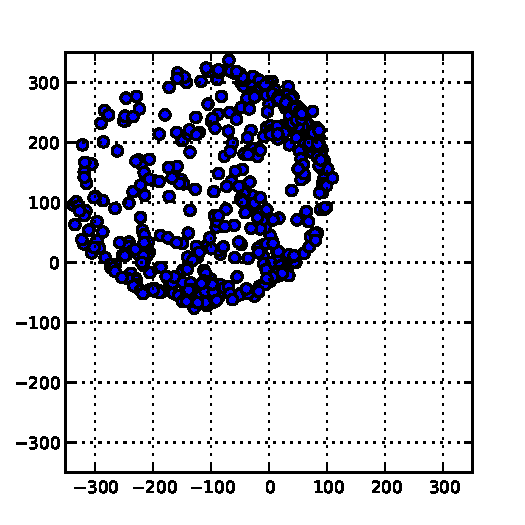
\includegraphics[width=0.45\textwidth]{img/zerocal_off.pdf}
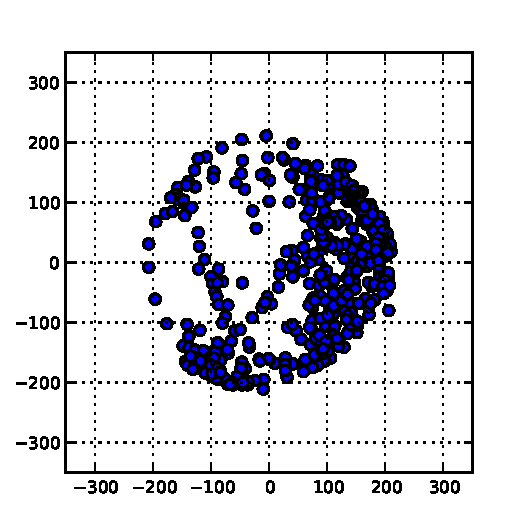
\includegraphics[width=0.45\textwidth]{img/zerocal_on.pdf}
\caption{Medições do sensor antes e depois da calibração do ``zero''}
\label{fig:zerocal}
\end{figure}


%\subsection{Problemas na comunicação com o sensor}
%\label{sub:problema_comunicacao_sensor}
%
%TODO: problema ao realizar muitas leituras muito rapidamente, cuja solução
%foi realizar leituras num timer.
%
%Citar também o "USB Reset".


%\subsection{Tamanho do firmware}
%\label{sub:firmware_size}
%
%Um desafio constante durante o projeto foi manter o tamanho do
%\textit{firmware} abaixo de 8192 bytes (tamanho da memória \textit{Flash}
%do microcontrolador, conforme descrito na seção \ref{sec:atmega8}), e,
%adicionalmente, abaixo de 6144 bytes (espaço total disponível após o uso do
%\textit{boot loader}, conforme seção \ref{sec:bootloader}).
%
%TODO: Dentre outras coisas, falar sobre as flags de compilação, que são
%específicas para a versão 4.5 do GCC.


\chapter{Transformação de coordenadas}
\label{cap:coordenadas}


\vfill{}
\begin{flushright}{}
``\emph{Models are a bunch of equations; physics is what happens when you
drop a hammer on your big toe. They are not the same. Just ask your big
toe.}''\\
{\small Ken Matusow}
\end{flushright}{\small \par}
\vfill{}

Neste capítulo é apresentado o problema de transformação de coordenadas, as
abordagens experimentadas e os resultados observados em cada abordagem.
\newpage


\section{Ferramentas auxiliares}
\label{sec:ferramentas}

O principal desafio teórico deste projeto foi transformar os vetores
tridimensionais lidos do sensor em coordenadas bidimensionais na tela do
computador. Não existe uma única solução para este problema e foi preciso
explorar algumas abordagens antes de decidir qual delas seria implementada
no microcontrolador.

Com o objetivo de experimentar e avaliar as diferentes abordagens para a
transformação de coordenadas, foram desenvolvidas algumas ferramentas
na linguagem Python. A escolha da linguagem foi motivada pela facilidade e
rapidez de se escrever protótipos e pela extensa e abrangente biblioteca
disponível.

A primeira ferramenta foi chamada de \texttt{generate\_sphere\_vectors.py} e
serve para simular leituras do sensor. Esta ferramenta imprime na saída
padrão uma lista de vetores 3D que cobrem pouco menos da metade da
superfície de uma esfera. Também imprime quatro vetores correspondentes aos
cantos da tela, os quais são usados nos cálculos explicados nas seções
\ref{sec:coord_geometria} e \ref{sec:coord_lineq}. A listagem
\ref{lst:generate_sphere_vectors} mostra um trecho da saída desta
ferramenta.

\begin{lstlisting}[numbers=none, float=h, label={lst:generate_sphere_vectors},
caption={Primeiras linhas da saída do programa \texttt{generate\_sphere\_vectors.py}}
]
topleft
172     69      75
topright
172     -69     75
bottomright
172     -69     -75
bottomleft
172     69      -75
0       141     141
2       141     141
5       141     141
7       141     141
10      141     141
\end{lstlisting}

A figura \ref{fig:half_sphere} mostra um gráfico dos vetores 3D
impressos por esta ferramenta. Esse gráfico corresponde à região de
\SIrange{-90}{90}{\degree} de longitude e \SIrange{-45}{45}{\degree} de
latitude. Há um espaçamento de \SI{1}{\degree} de longitude e
\SI{2}{\degree} de latitude entre os vetores.

\begin{figure}[h]
\centering
% ./generate_sphere_vectors.py -C | ./matplotlib_3d_plot.py -p -q -f 8 -s 3.5 3.5 -o ../monografia/img/half_sphere.png
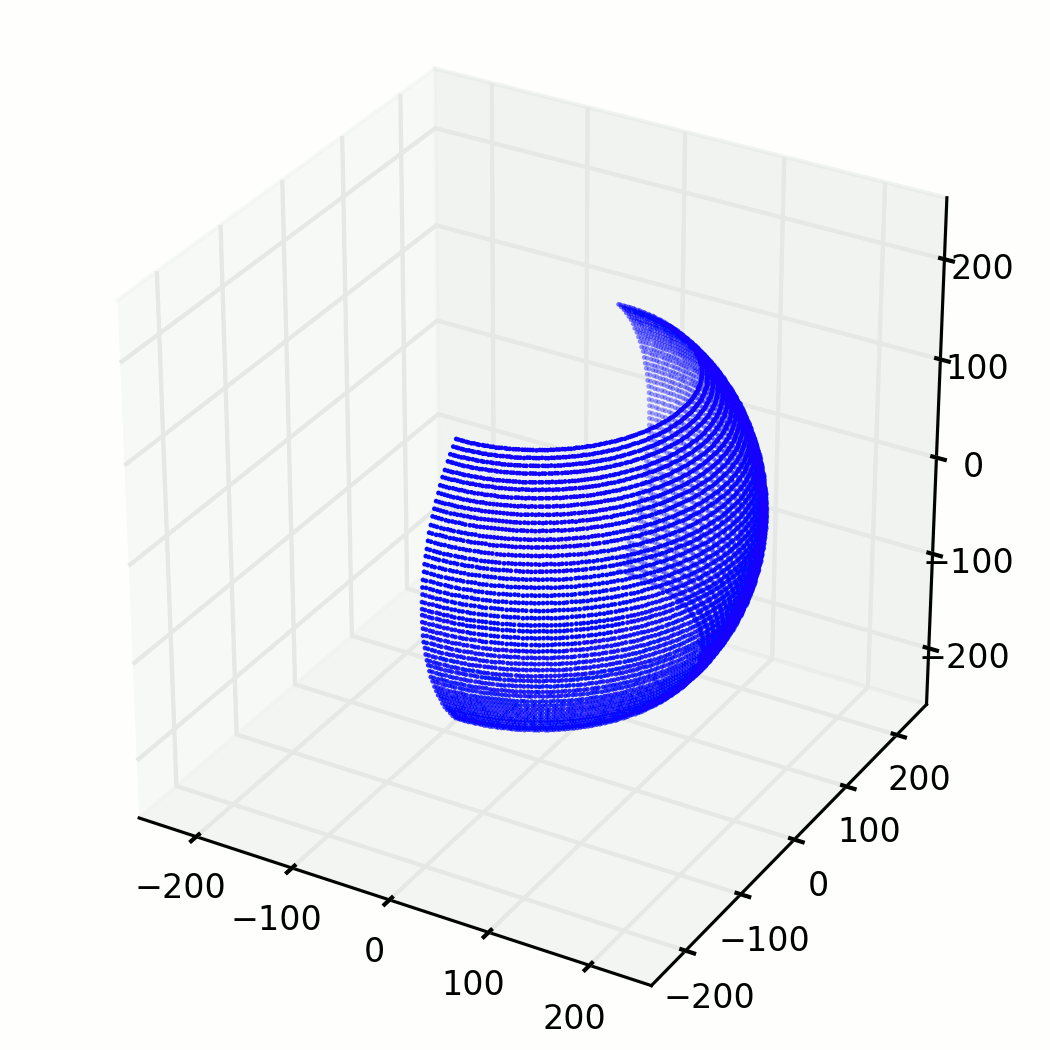
\includegraphics{img/half_sphere.png}
%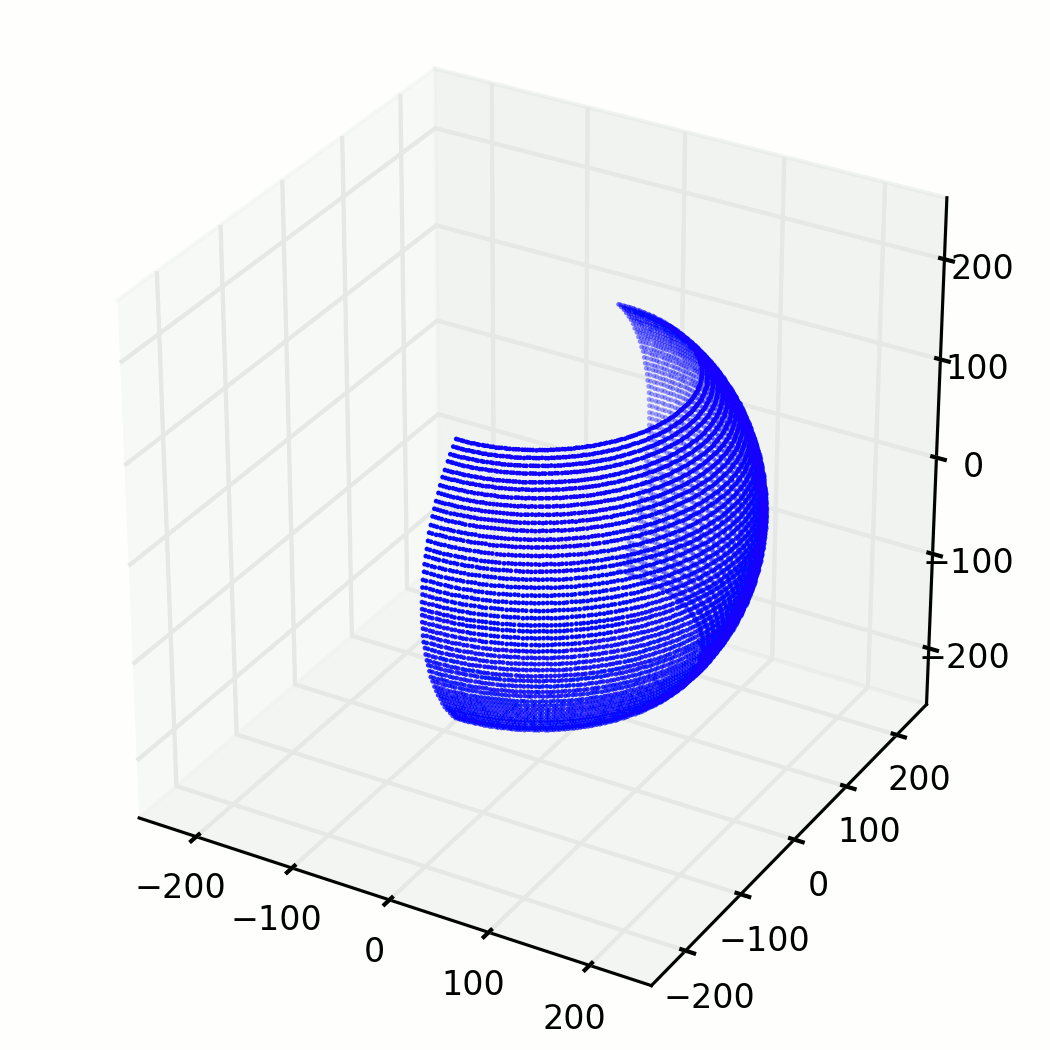
\includegraphics[width=0.5\textwidth]{img/half_sphere.png}
\caption{Visualização gráfica da saída do programa \texttt{generate\_sphere\_vectors.py}}
\label{fig:half_sphere}
\end{figure}

A segunda ferramenta foi chamada de \texttt{convert\_coordinates.py} e
implementa os algoritmos de transformação de coordenadas explicados nas
seções \ref{sec:coord_geometria} e \ref{sec:coord_lineq}. Esta ferramenta
lê vetores 3D a partir da entrada padrão e imprime na saída padrão as
coordenadas 2D correspondentes, calculadas de acordo com o algoritmo
selecionado. Um exemplo de entrada e saída para esta ferramenta pode ser
visto na listagem \ref{lst:convert_coordinates}

\begin{lstlisting}[numbers=none, float=h, label={lst:convert_coordinates},
caption={Entrada para o programa \texttt{convert\_coordinates.py} e a saída correspondente}
]
topleft
172     69      75
topright
172     -69     75
bottomright
172     -69     -75
bottomleft
172     69      -75
198     24      -3                      0.348924 0.517374
198     -3      24                      0.518884 0.36101
190     -44     45                      0.788635 0.228421
\end{lstlisting}

A terceira ferramenta foi chamada de \texttt{draw\_points.py} e serve para
visualizar graficamente as coordenadas 2D. Esta ferramenta desenha um ponto
na tela para cada par de coordenadas lido da entrada padrão. A figura
\ref{fig:draw_points} mostra a saída desta ferramenta para os três pontos da
listagem \ref{lst:convert_coordinates}.

\begin{figure}[h]
\centering
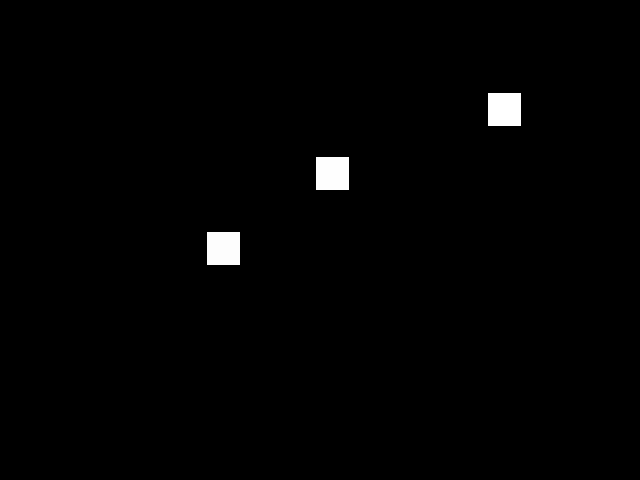
\includegraphics[width=0.5\textwidth]{img/draw_points_example.png}
\caption{Exemplo de saída do programa \texttt{draw\_points.py}}
\label{fig:draw_points}
\end{figure}

Essas três ferramentas podem ser usadas separadamente ou encadeadas através
de um \textit{pipeline}\footnote{
	\textit{Pipeline} significa ligar a saída padrão de um programa à
	entrada padrão do programa seguinte.
}.


\section{Transformação usando geometria}
\label{sec:coord_geometria}

Para esta abordagem é necessário calibrar os quatro cantos da tela, \ie,
definir quatro vetores no espaço tais que:

\begin{itemize}
\item O vetor $A$ aponta na direção do canto superior esquerdo da tela.
\item O vetor $B$ aponta na direção do canto superior direito da tela.
\item O vetor $C$ aponta na direção do canto inferior direito da tela.
\item O vetor $D$ aponta na direção do canto inferior esquerdo da tela.
\end{itemize}

Também é definido o vetor $P$ como sendo a direção apontada pelo usuário. O
objetivo da transformação de coordenadas é mapear o vetor $P$ em coordenadas
$(x, y)$ contidas no plano da tela do computador. As magnitudes dos vetores
não são importantes, apenas a direção é considerada. Todos esses vetores
podem ser vistos na figura \ref{fig:geometria_ABCD1}

\begin{figure}[h]
\centering
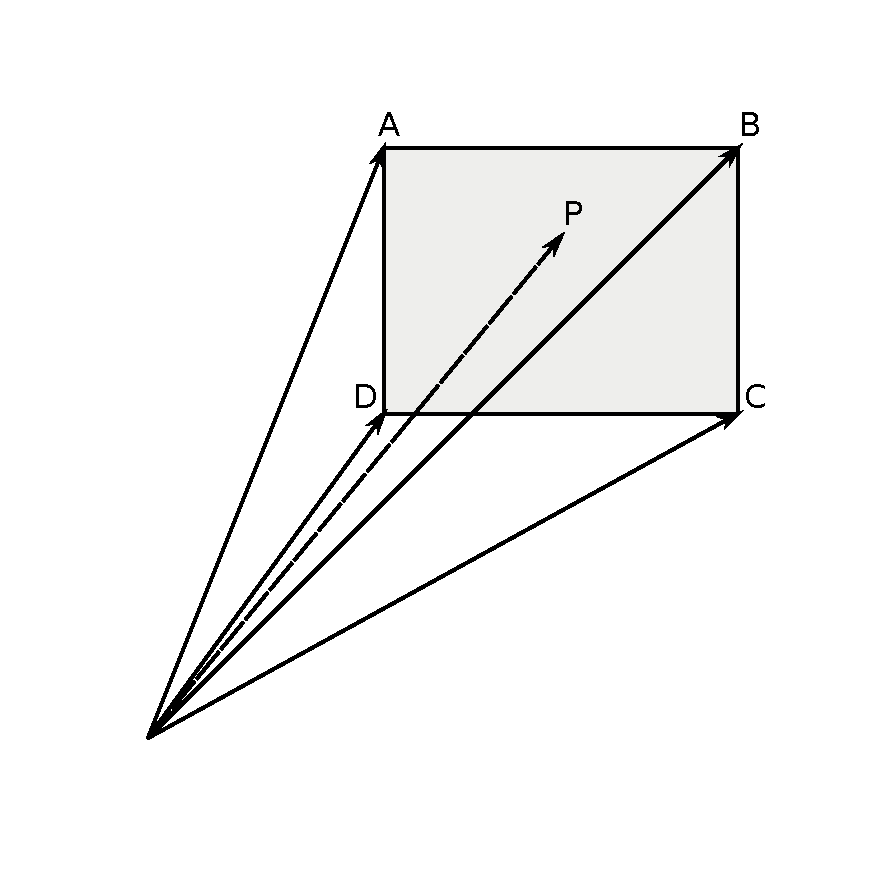
\includegraphics[width=0.5\textwidth]{img/geometria_ABCD1.pdf}
\caption{Definição dos vetores 3D}
\label{fig:geometria_ABCD1}
\end{figure}

Uma vez definido o problema, a etapa seguinte foi quebrá-lo em subproblemas.
Em vez de tentar calcular diretamente as coordenadas 2D relativas ao vetor
$P$, calcula-se a projeção de P em cada uma das bordas da tela, para a
seguir interpolar as coordenadas $(x, y)$ a partir das bordas, conforme a
figura \ref{fig:geometria_ABCD2}. Essa decisão foi tomada porque o
quadrilátero $ABCD$ não é necessariamente um retângulo.

\begin{figure}[h]
\centering
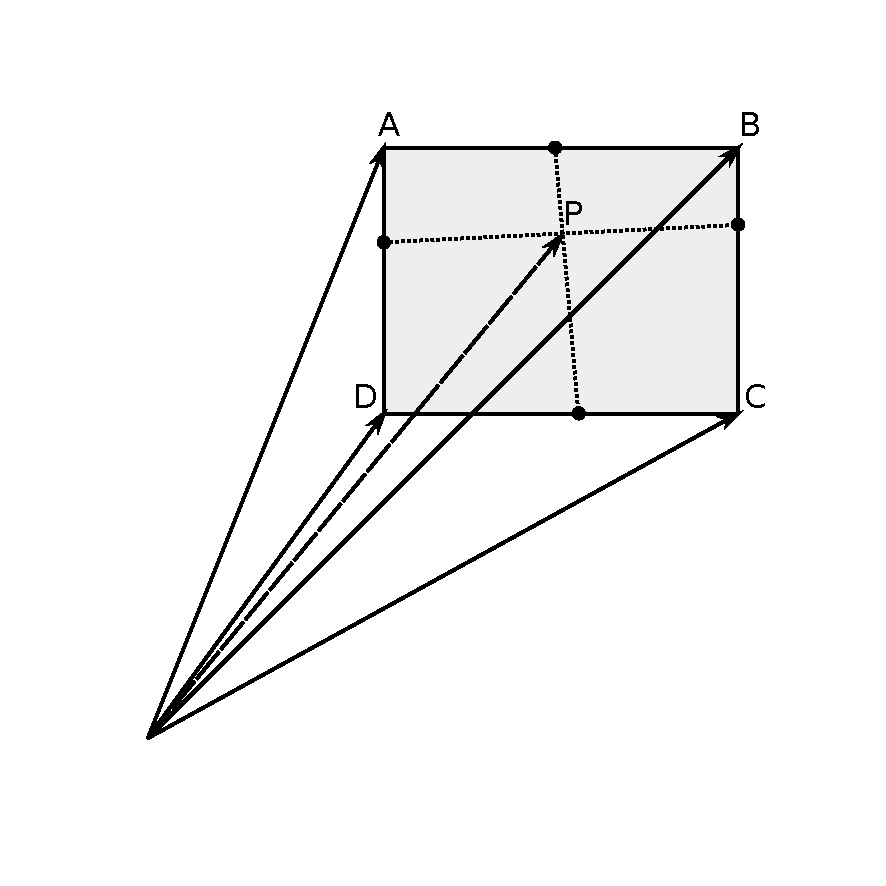
\includegraphics[width=0.5\textwidth]{img/geometria_ABCD2.pdf}
\caption{As coordenadas 2D podem ser interpoladas a partir da projeção de
$P$ em cada borda}
\label{fig:geometria_ABCD2}
\end{figure}

Para calcular essa projeção de $P$, primeiramente calcula-se o vetor
unitário $N$ \eqref{eq:normal}, normal ao plano de $A$ e $B$. São então
calculados $P_N$ \eqref{eq:Pnormal}, a componente de $P$ paralela ao vetor
$N$; e $P'$ \eqref{eq:Plinha}, a componente de $P$ contida no plano de $A$ e
$B$. Isso é ilustrado na figura \ref{fig:geometria_ABCD3}.

\begin{align}
\label{eq:normal}
N   & = \frac{A \times B}{ || A \times B || }   \\
\label{eq:Pnormal}
P_N & = (N \cdot P) N                           \\
\label{eq:Plinha}
P'  & = P - P_N
\end{align}

\begin{figure}[h]
\centering
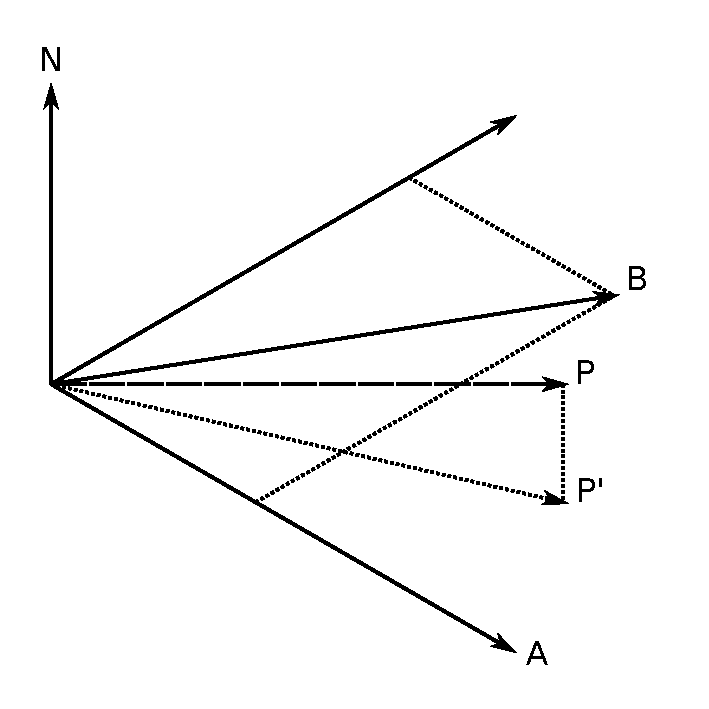
\includegraphics[width=0.5\textwidth]{img/geometria_ABCD3.pdf}
\caption{O vetor $P'$ é a componente de $P$ contida no plano de $A$ e $B$}
\label{fig:geometria_ABCD3}
\end{figure}

Uma vez tendo $P'$, a etapa final é calcular sua posição na borda delimitada
por $A$ e $B$. Essa posição é definida como um escalar $\alpha$ entre $0$ e
$1$, sendo que $0$ indica que $P'$ é coincidente com o vetor $A$, e $1$
indica que $P'$ é coincidente com o vetor $B$. Valores fora desse intervalo
indicam que $P'$ está fora do setor angular delimitado por $A$ e $B$.

Como $A$, $B$ e $P'$ estão no mesmo plano, o valor exato de $\alpha$ pode
ser calculado através de um sistema linear de duas variáveis $\alpha$ e
$\beta$, o qual pode ser representado com a equação vetorial
\eqref{eq:sistemaPlinhaVetorial}.

\begin{align}
\label{eq:sistemaPlinhaVetorial}
A   + \alpha (B-A)   & = \beta P'
\end{align}

As bases do espaço bidimensional correspondente ao plano dos vetores $A$,
$B$ e $P'$ podem ser definidas como os vetores $X$ e $Y$ ortonormais
\eqref{eq:sistemaPlinhaBases}. Todos os pontos desse plano podem ser
representados por uma combinação linear entre os vetores $X$ e $Y$.

\begin{align}
\label{eq:sistemaPlinhaBases}
X & = \frac{A}{ || A || }                     \\
Y & = \frac{A \times N}{ || A \times N || }   \nonumber
\end{align}

Definidas as bases do espaço bidimensional, as componentes de $A$, $(B-A)$ e
$P'$ nesse espaço podem ser calculadas usando produto interno.
\eqref{eq:sistemaPlinhaComponentes}

\begin{alignat}{2}
\label{eq:sistemaPlinhaComponentes}
A_X     & = A \cdot X     & \qquad A_Y     & = A \cdot Y      \\
(B-A)_X & = (B-A) \cdot X & \qquad (B-A)_Y & = (B-A) \cdot Y  \nonumber \\
P'_X    & = P' \cdot X    & \qquad P'_Y    & = P' \cdot Y     \nonumber
\end{alignat}

A equação vetorial \eqref{eq:sistemaPlinhaVetorial} pode ser reescrita
como duas equações escalares \eqref{eq:sistemaPlinhaEscalar}, utilizando as
componentes definidas em \eqref{eq:sistemaPlinhaComponentes}.

\begin{align}
\label{eq:sistemaPlinhaEscalar}
A_X + \alpha (B-A)_X & = \beta P'_X  \\
A_Y + \alpha (B-A)_Y & = \beta P'_Y  \nonumber
\end{align}

Por fim, resolvendo o sistema linear definido em
\eqref{eq:sistemaPlinhaVetorial} e \eqref{eq:sistemaPlinhaEscalar}, obtemos
o valor exato de $\alpha$ correspondente a uma das bordas da tela.

Repetindo os cálculos para as outras bordas, podemos calcular $(x,y)$
através de uma interpolação linear \eqref{eq:interpolacao_linear}.

\begin{align}
\label{eq:interpolacao_linear}
x(y) & = y (DC - AB) + AB  \\
y(x) & = x (BC - AD) + AD  \nonumber \\
x    & = \frac{AD  (DC - AB) + AB}{1 - (BC - AD)  (DC - AB)}  \nonumber \\
\intertext{onde}
AB, BC, DC, AD & = \text{valor de $\alpha$ para cada borda} \nonumber
\end{align}

Além do cálculo do valor exato de $\alpha$, também foram experimentados
cálculos aproximados para $\alpha$, usando
razão entre ângulos \eqref{eq:alpha_angulo},
razão entre distâncias \eqref{eq:alpha_dist},
razão entre senos \eqref{eq:alpha_sin},
razão entre cossenos \eqref{eq:alpha_cos},
razão entre tangentes \eqref{eq:alpha_tan}.
Os resultados de cada abordagem estão listados na seção
\ref{sec:coord_resultados}.

\begin{align}
\label{eq:alpha_angulo}
\alpha & = \frac{\angulo(A, P')}{\angulo(A, B)} \\
\label{eq:alpha_dist}
\alpha & = \frac{
		\left| \dfrac{A}{|A|} - \dfrac{P'}{|P'|} \right|
	}{
		\left| \dfrac{A}{|A|} - \dfrac{B }{|B |} \right|
	}  \\
\label{eq:alpha_sin}
\alpha & = \frac{\sin(\angulo(A, P'))}{\sin(\angulo(A, B))} \\
\label{eq:alpha_cos}
\alpha & = \frac{\cos(\angulo(A, P'))}{\cos(\angulo(A, B))} \\
\label{eq:alpha_tan}
\alpha & = \frac{\tan(\angulo(A, P'))}{\tan(\angulo(A, B))}
\end{align}

O ângulo entre dois vetores pode ser calculado como mostrado em
\eqref{eq:angulo}.

\begin{align}
\label{eq:angulo}
\angulo(A,B) & = \arccos( \cos(\theta) )    \\
             & = \arccos\left( \frac{A \cdot B}{|A||B|} \right)  \nonumber
\end{align}


\section{Transformação usando sistema de equações lineares}
\label{sec:coord_lineq}

Para esta abordagem é necessário calibrar três dos quatro cantos da tela.
São definidos três vetores no espaço tais que:

\begin{itemize}
\item O vetor $A$ aponta na direção do canto superior esquerdo da tela.
\item O vetor $B$ aponta na direção do canto superior direito da tela.
\item O vetor $D$ aponta na direção do canto inferior esquerdo da tela.
\end{itemize}

Também é definido o vetor $P$ como sendo a direção apontada pelo usuário.
Esta abordagem transforma o vetor $P$ diretamente em coordenadas $(x, y)$
contidas no plano da tela do computador através da solução de um sistema
linear de três variáveis.

Esse sistema decorre da observação de que qualquer ponto da tela pode ser
representado como ponto $A$ somado de um deslocamento horizontal na direção
$B-A$ e um deslocamento vertical na direção $D-A$, conforme figura
\ref{fig:lineq}.

\begin{figure}[h]
\centering
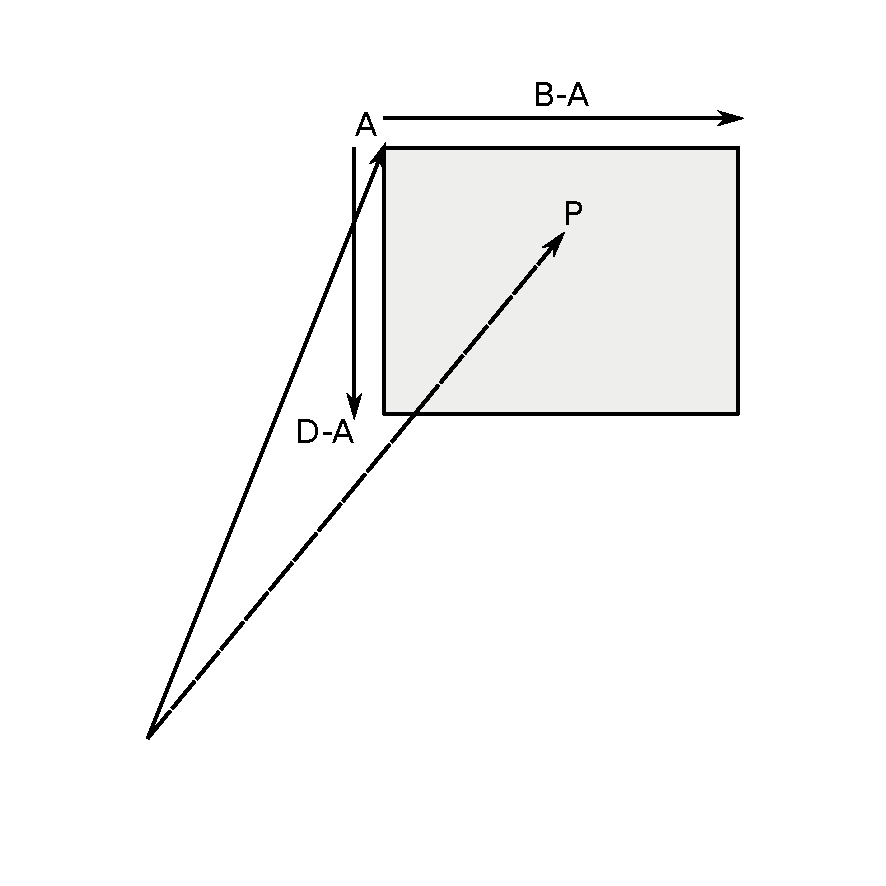
\includegraphics[width=0.5\textwidth]{img/lineq.pdf}
\caption{O vetor $P$ pode ser representado como $A + x(B-A) + y(D-A)$}
\label{fig:lineq}
\end{figure}

O sistema pode ser representado na forma vetorial conforme equações
\eqref{eq:lineq_inicial} e \eqref{eq:lineq_vetorial}. As coordenadas $(x,
y)$, já no plano da tela do computador, são a solução desse sistema. A
componente $z$ é descartada.

\begin{align}
\label{eq:lineq_inicial}
A + x (B-A) + y (D-A) & = z P  \\
\label{eq:lineq_vetorial}
x (B-A) + y (D-A) - z P & = -A
\end{align}

%Para melhores resultados nessa abordagem, a tela cujos três cantos são
%delimitados por $A$, $B$ e $D$ deve ter um formato de paralelogramo (ou um
%retângulo, que é um caso particular do paralelogramo).


\section{Resultados}
\label{sec:coord_resultados}

As abordagens descritas nas seções \ref{sec:coord_geometria} e
\ref{sec:coord_lineq} foram testadas experimentalmente usando o conjunto de
ferramentas da seção \ref{sec:ferramentas}.

Cada uma das abordagens foi testada cinco vezes usando o conjunto de vetores
gerados pela ferramenta \texttt{generate\_sphere\_vectors.py} -- ferramenta
descrita na seção \ref{sec:ferramentas}, cujos vetores estão representados
na figura \ref{fig:half_sphere} --, variando apenas a calibração do cantos
da tela entre cada teste. Isso permitiu analisar o comportamento de cada
algoritmo sob diferentes condições.

Os vetores de calibração escolhidos para cada teste possuem aberturas de
\SIlist{30;45;60;75;85}{\degree}, tanto na latitude como na longitude. Essa
abertura é ilustrada na figura \ref{fig:latitude_longitude}.

As figuras de \ref{fig:resultado_exact} a \ref{fig:resultado_lineq} mostram
o resultado de cada abordagem sendo testada com cada uma das cinco aberturas
citadas. Foram produzidas encadeando as três ferramentas auxiliares
descritas na seção \ref{sec:ferramentas} e mostram as deformações
introduzidas por cada abordagem, lembrando que o espaço entre os pontos é de
\SI{1}{\degree} horizontalmente e \SI{2}{\degree} verticalmente.

\begin{figure}[h]
\centering
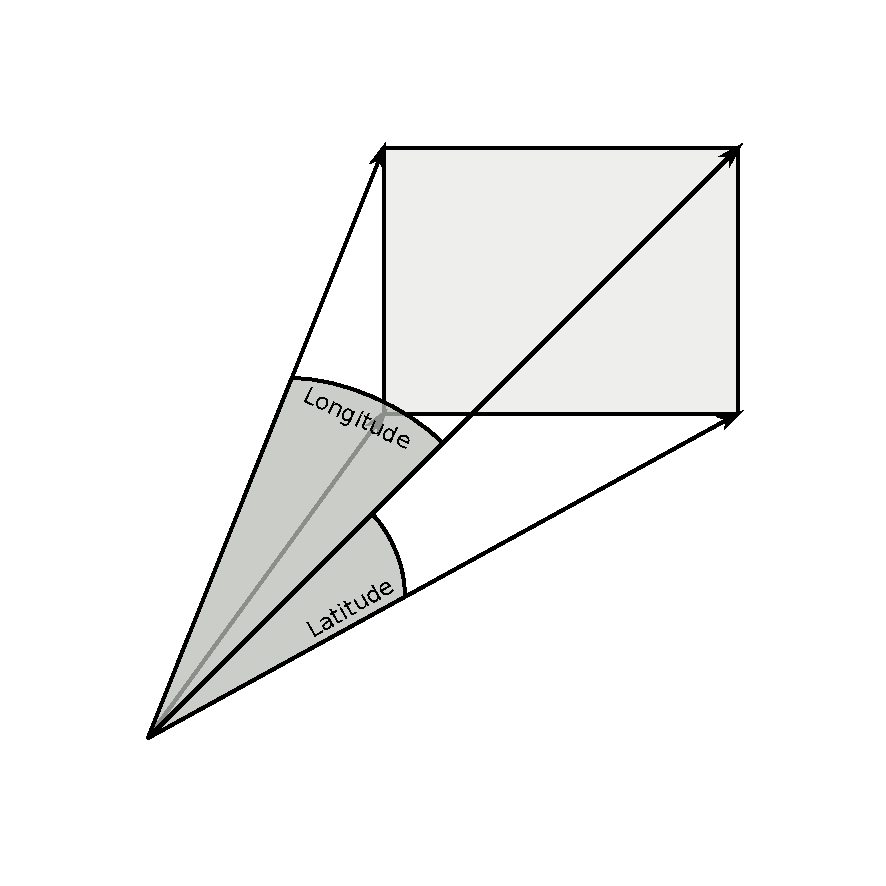
\includegraphics[width=0.5\textwidth]{img/latitude_longitude.pdf}
\caption{Os dois ângulos de abertura para os vetores de calibração}
\label{fig:latitude_longitude}
\end{figure}

\begin{figure}
\centering
\resultadoimagens{12}
\caption{Cálculo exato de $\alpha$}
\label{fig:resultado_exact}
\end{figure}

\begin{figure}
\centering
\resultadoimagens{7}
\caption{Razão entre ângulos}
\label{fig:resultado_angulo}
\end{figure}

\begin{figure}
\centering
\resultadoimagens{11}
\caption{Razão entre distâncias}
\label{fig:resultado_dist}
\end{figure}

\begin{figure}
\centering
\resultadoimagens{9}
\caption{Razão entre senos}
\label{fig:resultado_sin}
\end{figure}

%\clearpage

\begin{figure}
\centering
\resultadoimagens{8}
\caption{Razão entre cossenos}
\label{fig:resultado_cos}
\end{figure}

\begin{figure}
\centering
\resultadoimagens{10}
\caption{Razão entre tangentes}
\label{fig:resultado_tan}
\end{figure}

\begin{figure}
\centering
\resultadoimagens{13}
\caption{Sistema linear de 3 variáveis}
\label{fig:resultado_lineq}
\end{figure}

É possível observar que, com exceção da razão entre cossenos
(\ref{fig:resultado_cos}), todas as abordagens tiveram um bom resultado para
aberturas pequenas, de até \SI{30}{\degree} ou \SI{45}{\degree}. As
distorções somente são acentuadas para aberturas maiores, a partir de
\SI{30}{\degree} ou \SI{60}{\degree}.

A razão entre ângulos (\ref{fig:resultado_angulo}) e a razão entre
distâncias (\ref{fig:resultado_dist}) apresentaram comportamentos muito
parecidos. A região central da tela sofreu pouca deformação, enquanto as
regiões próximas das bordas apresentaram distorções bastante acentuadas.

A razão entre senos (\ref{fig:resultado_sin}) apresentou um comportamento
próximo da razão entre ângulos e da razão entre distâncias, porém com
deformações mais acentuadas tanto na região central como na região
periférica.

As coordenadas transformadas usando a razão entre cossenos
(\ref{fig:resultado_cos}) apresentaram uma rotação de
\SIrange{15}{25}{\degree} em todas as aberturas testadas. Por outro lado,
foi a abordagem com menor distorção nas bordas.

A razão entre tangentes (\ref{fig:resultado_tan}) só obteve bons resultados
para aberturas pequenas. Para aberturas maiores, as distorções são
extremamente acentuadas. Isso não é surpresa, visto que a função tangente
tende para o infinito quando a abertura tende para \SI{90}{\degree}.

O cálculo exato do escalar $\alpha$ obteve o melhor resultado geral,
apresentando muito pouca deformação na região central assim como uma área de
distorções periféricas relativamente pequena, significativamente menor que a
área das outras abordagens.

Por fim, a abordagem usando um sistema linear de três equações
(\ref{fig:resultado_lineq}) apresentou distorções cada vez mais acentuadas
conforme os ângulos de abertura ficavam maiores. Essas distorções ocorrem
por se mapear uma região da esfera num plano, e portanto são relativamente
pequenas quando a região da esfera é suficientemente reduzida.


\chapter{Conclusões}
\label{cap:conclusoes}


\vfill{}
\begin{flushright}{}
``\emph{
	This was a triumph.    \\
	I'm making a note here:\\
	HUGE SUCCESS.          \\
	It's hard to overstate \\
	my satisfaction.
}''\\
{\small Jonathan Coulton} \\
{\small Música final do jogo \textit{Portal}}
\end{flushright}{\small \par}
\vfill{}

Neste capítulo são apresentados os resultados alcançados, as limitações
encontradas e sugestões para trabalhos futuros.
\newpage


\section{Resultados alcançados}
\label{sec:resultados}

De maneira geral, o projeto obteve grande sucesso em seus objetivos. O
dispositivo funciona como esperado e é fácil de usar.

O \textit{boot loader} (seção \ref{sec:bootloader}) se mostrou extremamente
prático durante o desenvolvimento, e é uma excelente ferramenta para ser
usada em projetos futuros.

O \textit{driver} V-USB (seção \ref{sec:vusb}) se confirmou como uma opção
bastante prática para desenvolver dispositivos \ac{USB} \textit{low speed}.
A implementação de um \ac{USB} \ac{HID} neste projeto funcionou como
esperado: o comportamento foi \textit{plug-and-play}, funcionando
imediatamente nos sistemas operacionais testados -- Linux, Mac OS X e
Windows -- sem precisar de qualquer intervenção manual.

A escolha de um microcontrolador AVR também foi bem sucedida, considerando a
quantidade e a qualidade das ferramentas disponíveis para essa arquitetura.

Por outro lado, a escolha do microcontrolador ATmega8 foi um pouco
restritiva devido à sua memória \textit{Flash} relativamente pequena. Foi
necessário desabilitar partes do \textit{firmware} durante o
desenvolvimento para que ele pudesse coexistir com o \textit{boot loader} na
memória. Ao final do projeto, alguns itens menos importantes do menu de
configurações foram desabilitados para que o \textit{firmware} pudesse caber
inteiro na memória.

Apesar da implementação de um menu (seção \ref{sec:menu}) ter aumentado
substancialmente o tamanho do \textit{firmware}, ele foi fundamental para
tornar intuitiva a configuração dos parâmetros do dispositivo. Dado que se
tenha espaço suficiente, pode-se até incluir instruções de uso no sistema de
menus, dispensando quase que totalmente a necessidade de um manual de
instruções para o usuário.

%O \textit{driver} de comunicação \ac{I2C} (seção \ref{sec:twi}) foi bastante
%prático de usar, porém sua rotina de interrupção precisa ser melhorada

%O método usado para conversão de coordenadas não é perfeito, mas atende às
%necessidades.

Limitações nas medidas do sensor puderam ser observadas como oscilações na
posição do ponteiro do \textit{mouse}. Mesmo depois de implementado um
algoritmo de suavização (seção \ref{sub:mouse_smoothing}), o ponteiro ainda
oscilava de maneira perceptível, embora com amplitude bastante reduzida.

Por fim, o uso individual de um magnetômetro para controlar o ponteiro do
\textit{mouse} possui suas limitações. Como o campo magnético da Terra é
aproximadamente paralelo à superfície (exceto nos pólos), o dispositivo
deste projeto só funciona satisfatoriamente se o usuário estiver de frente
para o Norte ou para o Sul. Caso o usuário esteja de frente para o Leste ou
Oeste, os movimentos verticais serão altamente comprometidos. Isso acontece
porque esse tipo de movimento será provocado por uma rotação do sensor num
eixo paralelo ao campo magnético, e esse tipo de movimento não causa
variação na leitura do sensor (ou causa uma variação muito pequena).


\section{Trabalhos futuros}
\label{sec:trabalhos_futuros}

Apesar deste projeto funcionar como esperado, ainda pode ser refinado de
várias formas.

A comunicação com o sensor foi implementada usando um conjunto de fios e o
protocolo \ac{I2C}. Substituir essa interface por uma comunicação sem fio
tornaria o dispositivo muito mais prático para o usuário.

O sensor usado neste projeto, conforme descrito na seção
\ref{sub:software_sensor_config}, permite no máximo 75 medições por segundo
no modo de medição contínua. Seria possível alcançar até 160 medições por
segundo caso a \ac{PCB} onde o sensor foi colocado tivesse um contato para o
pino DRDY, como mostra a figura \ref{fig:loveelectronics_photos}.

\begin{figure}[h]
\centering
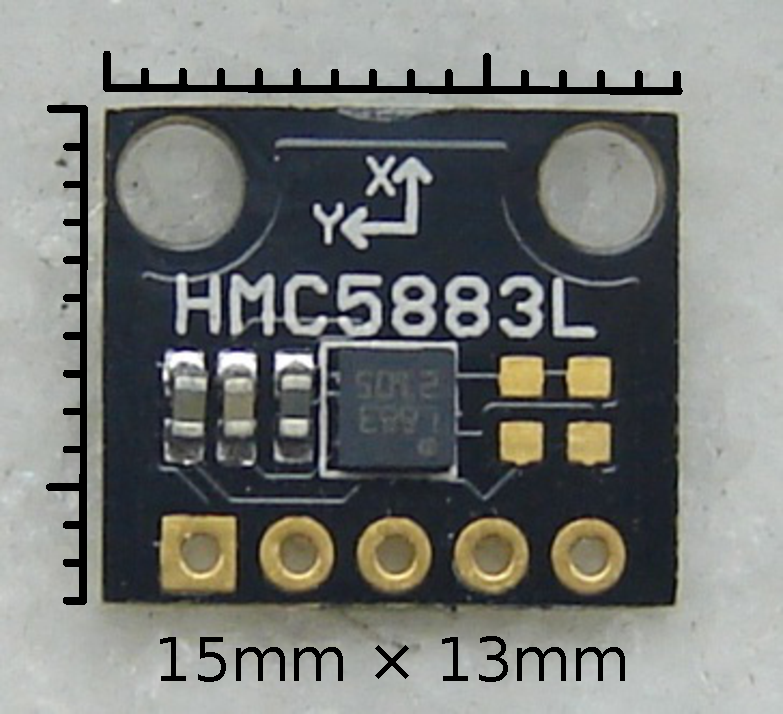
\includegraphics[width=0.45\textwidth]{img/sensor_other_pcb_front.pdf}
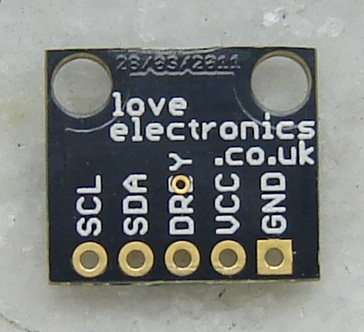
\includegraphics[width=0.45\textwidth]{img/sensor_other_pcb_back.jpg}
\caption{Fotos de uma PCB com cinco contatos disponíveis}
\label{fig:loveelectronics_photos}
\end{figure}

Outra opção de trabalho futuro é trocar o sensor HMC5883L por algum outro
com medições mais precisas. Isso tem potencial de diminuir as oscilações do
ponteiro, aumentando a precisão durante o uso do dispositivo.

Podem ainda ser feitos estudos teóricos e experimentais sobre diferentes
algoritmos de transformação de coordenadas. Com um microcontrolador com mais
memória, seria possível implementar algoritmos mais complexos.

Finalmente, a adição de um segundo sensor do tipo acelerômetro ou giroscópio
eliminaria a restrição de estar virado para o Norte ou para o Sul. Seria
necessário estudar novas abordagens para a transformação de coordenadas,
visto que as abordagens investigadas neste projeto utilizam dados vindos de
apenas um sensor.


%%fakesection  Bibliografia

\bibliographystyle{abnt-num}
\bibliography{mouse_magnetometro_monografia}

% How to add \url{} to "url=" entries from Pybliographic:
% :%s/\(url\s*=\s*{\)\([^\\].*[^}]\)\(},\?\)/\1\\url{\2}\3/


%%fakesection  Apendice
\apendice


\chapter{\texttt{main.c}}
\label{ape:main}
\lstinputlisting[language=C, lineskip=-0.4\baselineskip]{codigofonte/main.c}

\chapter{\texttt{buttons.h} e \texttt{buttons.c}}
\label{ape:buttons}
\lstinputlisting[language=C, lineskip=-0.4\baselineskip]{codigofonte/buttons.h}
\clearpage
\lstinputlisting[language=C, lineskip=-0.4\baselineskip]{codigofonte/buttons.c}

\chapter{\texttt{common.h}}
\label{ape:common}
\lstinputlisting[language=C, lineskip=-0.4\baselineskip]{codigofonte/common.h}

\chapter{\texttt{int\_eeprom.h} e \texttt{int\_eeprom.c}}
\label{ape:int_eeprom}
\lstinputlisting[language=C, lineskip=-0.4\baselineskip]{codigofonte/int_eeprom.h}
\clearpage
\lstinputlisting[language=C, lineskip=-0.4\baselineskip]{codigofonte/int_eeprom.c}

\chapter{\texttt{keyemu.h} e \texttt{keyemu.c}}
\label{ape:keyemu}
\lstinputlisting[language=C, lineskip=-0.4\baselineskip]{codigofonte/keyemu.h}
\clearpage
\lstinputlisting[language=C, lineskip=-0.4\baselineskip]{codigofonte/keyemu.c}

\chapter{\texttt{menu.h} e \texttt{menu.c}}
\label{ape:menu}
\lstinputlisting[language=C, lineskip=-0.4\baselineskip]{codigofonte/menu.h}
\clearpage
\lstinputlisting[language=C, lineskip=-0.4\baselineskip]{codigofonte/menu.c}

\chapter{\texttt{mouseemu.h} e \texttt{mouseemu.c}}
\label{ape:mouseemu}
\lstinputlisting[language=C, lineskip=-0.4\baselineskip]{codigofonte/mouseemu.h}
\clearpage
\lstinputlisting[language=C, lineskip=-0.4\baselineskip]{codigofonte/mouseemu.c}

\chapter{\texttt{sensor.h} e \texttt{sensor.c}}
\label{ape:sensor}
\lstinputlisting[language=C, lineskip=-0.4\baselineskip]{codigofonte/sensor.h}
\clearpage
\lstinputlisting[language=C, lineskip=-0.4\baselineskip]{codigofonte/sensor.c}

\chapter{\texttt{hardwareconfig.h} e \texttt{usbconfig.h}}
\label{ape:usbconfig}
\lstinputlisting[language=C, lineskip=-0.4\baselineskip]{codigofonte/hardwareconfig.h}
\clearpage
\lstinputlisting[language=C, lineskip=-0.4\baselineskip]{codigofonte/usbconfig.h}

\chapter{\texttt{Makefile}}
\label{ape:makefile}
\lstinputlisting[language=make, lineskip=-0.4\baselineskip]{codigofonte/Makefile}

%\lstinputlisting[language=C, lineskip=-0.4\baselineskip]{../firmware/avr315/TWI_Master.h}
%\lstinputlisting[language=C, lineskip=-0.4\baselineskip]{../firmware/avr315/TWI_Master.c}


\chapter{\texttt{generate\_sphere\_vectors.py}}
\label{ape:generate_sphere_vectors}
\lstinputlisting[language=Python, lineskip=-0.4\baselineskip]{codigofonte/generate_sphere_vectors.py}

\chapter{\texttt{convert\_coordinates.py}}
\label{ape:convert_coordinates}
\lstinputlisting[language=Python, lineskip=-0.4\baselineskip]{codigofonte/convert_coordinates.py}

\chapter{\texttt{draw\_points.py}}
\label{ape:draw_points}
\lstinputlisting[language=Python, lineskip=-0.4\baselineskip]{codigofonte/draw_points.py}

\chapter{\texttt{render\_images.sh}}
\label{ape:render_images}
\lstinputlisting[language=bash, lineskip=-0.4\baselineskip]{codigofonte/render_images.sh}


%%fakesection  Anexo
\anexo


\chapter{ATmega8 datasheet}
\label{anx:atmega8_datasheet}

Páginas            1-6, 9-10, 17-19, 157-160, 168-170, 213, 216-217 \cite{ATmega8}.

\includepdf[pages={1-6, 9-10, 17-19, 157-160, 168-170, 213, 216-217}]{/home/denilson/avr/PDFs/doc2486.pdf}


\chapter{HMC5883L datasheet}
\label{anx:hmc5883l_datasheet}

Todas as páginas \cite{HMC5883L}.

\includepdf[pages={-}]{../../hmc5883/HMC5883L.pdf}


\chapter{3V Tips 'n Tricks}
\label{anx:3vtipsandtricks_pdf}

Páginas 1, 4 \cite{3vtipsandtricks}.

\includepdf[pages={1, 4}]{../../level-shifting/en026368.pdf}


\chapter{Bi-directional level shifter for I²C-bus and other systems}
\label{anx:AN97055_pdf}

Páginas 8-12 \cite{AN97055}.

\includepdf[pages={8-12}]{../../level-shifting/AN97055.pdf}


\chapter{Level shifting techniques in I²C-bus design}
\label{anx:AN10441_pdf}

Páginas 3-4 \cite{AN10441}.

\includepdf[pages={3-4}]{../../level-shifting/AN10441.pdf}


%\chapter{AVR315: Using the TWI module as I²C master}
%\label{anx:avr315_pdf}
%
%Todas as páginas \cite{AVR315}.
%
%\includepdf[pages=-]{/home/denilson/avr/PDFs/doc2564.pdf}


\end{document}

% vim:filetype=tex ts=4 sw=4 noet tw=76
